% FORMAT AND PACKAGES
% {
\documentclass[a4paper, 11pt]{article}
\usepackage{a4wide,amssymb,epsfig,latexsym,multicol,array,hhline,fancyhdr}
\usepackage{vntex}
\usepackage{amsmath}
\usepackage{lastpage}
\usepackage[lined,boxed,commentsnumbered]{algorithm2e}
\usepackage{enumerate}
\usepackage{xcolor}
\usepackage{xltabular}
\usepackage{graphicx}              % Standard graphics package
\usepackage{array}
\usepackage{tabularx, caption}
\usepackage{multirow}
\usepackage{multicol}
\usepackage{rotating}
\usepackage{graphics}
\usepackage{geometry}
\usepackage{setspace}
\usepackage{epsfig}
\usepackage{tikz}
\usepackage{xfrac}
\usepackage{bm}
\usepackage{biblatex}
\usepackage[colorlinks]{hyperref}
% \usepackage[acronym,toc]{glossaries}
% \usepackage[symbols,nogroupskip,nonumberlist]{glossaries-extra}
\usepackage[
  sort=none,% no sorting or indexing required
  abbreviations,% create list of abbreviations
  symbols,% create list of symbols
  stylemods,style=list, % set the default glossary style
  nogroupskip, nonumberlist, nomain
]{glossaries-extra}

% FORMATTING
% {
\DeclareMathOperator{\arccot}{arccot}
\captionsetup[table]{name=Bảng}
\captionsetup[figure]{name=Hình}
\newenvironment{Description}{\list{}{%
    \let\makelabel\descriptionlabel    % this comes from the original description environment
    \setlength{\rightmargin}{\leftmargin}% this comes from the original quote environment
    \setlength{\labelwidth}{0pt}%          this is new
}}{\endlist}

\addbibresource{citations.bib}

\hypersetup{urlcolor=blue,linkcolor=black,citecolor=black,colorlinks=true}
\usetikzlibrary{arrows,snakes,backgrounds}
\definecolor{mathblue}{RGB}{0,114,188}
% \makeatletter  \def\m@th{\mathsurround\z@\color{mathblue}} \makeatother
% \everymath{\color{mathblue}}
% \setmathfont[Color=000000]{Arial}
%\usepackage{pstcol}                 % PSTricks with the standard color package
\newtheorem{theorem}{{\bf Theorem}}
\newtheorem{property}{{\bf Property}}
\newtheorem{proposition}{{\bf Proposition}}
\newtheorem{corollary}[proposition]{{\bf Corollary}}
\newtheorem{lemma}[proposition]{{\bf Lemma}}

\AtBeginDocument{\renewcommand{\listfigurename}{Danh sách hình ảnh}}
\AtBeginDocument{\renewcommand{\listtablename}{Danh sách bảng}}
\AtBeginDocument{\renewcommand*\contentsname{Mục lục}}
\AtBeginDocument{\renewcommand*\refname{References}}
%\usepackage{fancyhdr}

\setlength{\headheight}{40pt}
\pagestyle{fancy}
\fancyhead{} % clear all header fields
\fancyhead[L]{
  \begin{tabular}{rl}
    \begin{picture}(25,15)(0,0)
      \put(0,-8){
\includegraphics[width=8mm, height=8mm]{image/hcmut.png}}
      %\put(0,-8){\epsfig{width=10mm,figure=hcmut.eps}}
    \end{picture}&
    %\includegraphics[width=8mm, height=8mm]{hcmut.png} & %
    \begin{tabular}{l}
      \textbf{\bf \ttfamily Trường Đại học Bách khoa - ĐHQG-HCM}\\
      \textbf{\bf \ttfamily Khoa Khoa học và Kỹ thuật Máy tính}
    \end{tabular}
  \end{tabular}
}
\fancyhead[R]{
  \begin{tabular}{l}
    \tiny \bf \\
    \tiny \bf
\end{tabular}  }
\fancyfoot{} % clear all footer fields
\fancyfoot[L]{\scriptsize \ttfamily Bài tập lớn Kho dữ liệu và hệ hỗ trợ quyết định - Năm học 2026 - 2027}
\fancyfoot[R]{\scriptsize \ttfamily Trang {\thepage}/\pageref{LastPage}}
\renewcommand{\headrulewidth}{0.3pt}
\renewcommand{\footrulewidth}{0.3pt}

\setcounter{secnumdepth}{4}
\setcounter{tocdepth}{4}

\makeatletter
\newcounter {subsubsubsection}[subsubsection]
\renewcommand\thesubsubsubsection{\thesubsubsection .\@alph\c@subsubsubsection}
\newcommand\subsubsubsection{\@startsection{subsubsubsection}{4}{\z@}%
  {-3.25ex\@plus -1ex \@minus -.2ex}%
  {1.5ex \@plus .2ex}%
{\normalfont\normalsize\bfseries}}
\newcommand*\l@subsubsubsection{\@dottedtocline{3}{10.0em}{4.1em}}
\newcommand*{\subsubsubsectionmark}[1]{}
% \def\m@th{\mathsurround\z@\color{mathblue}}
\makeatother
% }
% }

% ACRONYMS & SYMBOLS
% {
% \makeglossaries
\setabbreviationstyle{long-short}
\newabbreviation{ode}{ODE}{(First-Order) Ordinary Differential Equation}
\newabbreviation{ivp}{IVP}{Initial-Value Problem}
\newabbreviation{lte}{LTE}{Local Truncation Error}
\newabbreviation{ds}{DS}{Dynamical System}
\newabbreviation{fig}{Fig.}{Figure}
\newabbreviation{tab}{Tab.}{Table}
\newabbreviation{sys}{Sys.}{System of Equations}
\newabbreviation{eq}{Eq.}{Equation}
\newabbreviation{eg}{e.g.}{For Example}
\newabbreviation{ie}{i.e.}{That Is}
% \glsnoexpandfields
\glsxtrnewsymbol[description = {Set of natural numbers}]{natural}{\ensuremath{\mathbb{N}}}
\glsxtrnewsymbol[description = {Set of real numbers}]{real}{\ensuremath{\mathbb{R}}}
\glsxtrnewsymbol[description = {Set of positive real numbers}]{real_positive}{\ensuremath{\mathbb{R}^+}}

% }

% Code listing
\usepackage{listings}
% \usepackage{xcolor}
\definecolor{codegreen}{rgb}{0,0.6,0}
\definecolor{codegray}{rgb}{0.5,0.5,0.5}
\definecolor{codepurple}{rgb}{0.58,0,0.82}
\definecolor{backcolour}{rgb}{0.95,0.95,0.92}

\lstdefinestyle{mystyle}{
  backgroundcolor=\color{backcolour},
  commentstyle=\color{codegreen},
  keywordstyle=\color{magenta},
  numberstyle=\tiny\color{codegray},
  stringstyle=\color{codepurple},
  basicstyle=\ttfamily\footnotesize,
  breakatwhitespace=false,
  breaklines=true,
  captionpos=b,
  keepspaces=true,
  numbers=left,
  numbersep=5pt,
  showspaces=false,
  showstringspaces=false,
  showtabs=false,
  tabsize=2
}

\lstset{style=mystyle}
%

% Float [H]
\usepackage{float}
%

% DOCUMENT
\begin{document}

% TITLE PAGE
\begin{titlepage}
  \begin{center}
    ĐẠI HỌC QUỐC GIA THÀNH PHỐ HỒ CHÍ MINH \\
    TRƯỜNG ĐẠI HỌC BÁCH KHOA \\
    KHOA KHOA HỌC VÀ KỸ THUẬT MÁY TÍNH
  \end{center}

  \vspace{1cm}

  \begin{figure}[h!]
    \begin{center}
      
\includegraphics[width=3cm]{image/hcmut.png}
    \end{center}
  \end{figure}

  \vspace{1cm}
% Kho dữ liệu và hệ hỗ trợ quyết định
  \begin{center}
    \begin{tabular}{c}
      \multicolumn{1}{l}{\textbf{{\Large KHO DỮ LIỆU VÀ HỆ HỖ TRỢ RA QUYẾT ĐỊNH}}} \\
      ~~                                                                   \\
      \hline
      \\
      \multicolumn{1}{l}{\textbf{{\Large Assignment (CO4031)}}}                    \\
      \\
      \textbf{\textit{{\Huge Data Warehouse }}}  \\
      \textbf{\textit{{\Huge And Decision Support System}}} \\
      \textbf{\textit{{\Huge for Marketing }}} \\
      \\
      \hline
    \end{tabular}
  \end{center}

  \vspace{2cm}

  \begin{table}[h]
    \centering
    \begin{tabular}{rl}
      \hspace{3 cm}\textbf{Giảng viên hướng dẫn}:
      & Võ Thị Ngọc Châu \\
      &                  \\[10pt]
      \textbf{Sinh viên thực hiện}: & Nguyễn Xuân Huy Hoàng - 2311070 \\
      & Trần Vĩnh Dũng - 2310574 \\
      & Bùi Trọng Hiển - 2310993 \\
    \end{tabular}
  \end{table}

  \begin{center}
    {\footnotesize THÀNH PHỐ HỒ CHÍ MINH, 10/2026}
  \end{center}
\end{titlepage}

\pagebreak
\tableofcontents
\pagebreak

% % Glossaries
% % {}
% \printunsrtglossary[type={symbols}, title={Danh sách ký hiệu}]
% \printunsrtglossary[type={abbreviations}, title={Danh sách từ viết tắt}]
\pagebreak
\listoffigures
\listoftables
\pagebreak
\addcontentsline{toc}{section}{\listfigurename}
\addcontentsline{toc}{section}{\listtablename}

% }

% Member list
\section*{Danh sách thành viên \& phân công}
\addcontentsline{toc}{section}{Danh sách thành viên \& phân công}
\begin{center}
  \begin{table}[h]
    \centering
    \begin{tabular}{|c|c|c|l|c|}
      \hline
      \textbf{STT}       & \textbf{Họ và tên}                & \textbf{MSSV}            & \textbf{Phân công} & \textbf{\% hoàn thành} \\
      \hline
      %%%%%Student 1%%%%%%%%%%
      \multirow{3}{*}{1} & \multirow{3}{*}{Bùi Trọng Hiển}    & \multirow{3}{*}{2310993} &
      - placeholder  & \multirow{3}{*}{100\%}                                                                                     \\
      &                                   &                          & - ...       &                        \\
      &                                   &                          & - ...  &                        \\
      \hline
      %%%%%Student 2%%%%%%%%%%%
      \multirow{2}{*}{2} & \multirow{2}{*}{Nguyễn Xuân Huy Hoàng}  & \multirow{2}{*}{2311070} &
      - placeholder  & \multirow{2}{*}{100\%}  \\
      &    &   & - placeholder &   \\
      \hline
      %%%%%Student 3%%%%%%%%%%% 
      \multirow{3}{*}{3} & \multirow{3}{*}{Trần Vĩnh Dũng} & \multirow{3}{*}{2310574} &
      - placeholder & \multirow{3}{*}{100\%}                                                                                     \\
      &                                   &                          & - ...       &                        \\
      &                                   &                          & - ...           &                        \\
      \hline
      
    \end{tabular}
    \caption{\label{table1}Danh sách thành viên \& phân công}
  \end{table}
\end{center}

\pagebreak

% \begin{figure}[H]
%   \centering
%   
\includegraphics[width=0.5\linewidth]{image/hcmut.png}
%   \caption{Red-black tree}
%   \label{fig:enter-label}
% \end{figure}

\pagebreak
\section{Giới thiệu}
\subsection{Bối cảnh}
Trong môi trường kinh doanh hiện đại, Marketing số không chỉ là hoạt động quảng cáo, truyền thông hay bán hàng, mà còn là quá trình thu thập dữ liệu, phân tích hành vi khách hàng, đánh giá hiệu quả chiến dịch và phân bổ nguồn lực nhằm đạt được mục tiêu kinh doanh. Doanh nghiệp có thể sử dụng nhiều kênh như Google Ads, Meta/Facebook Ads, TikTok Ads, email marketing và các nền tảng quảng bá khác. Mỗi nền tảng tạo ra dữ liệu về chi phí quảng cáo, lượt hiển thị, lượt nhấp, chuyển đổi, tương tác và doanh thu được ghi nhận theo mô hình phân bổ của nền tảng.\medskip

Thông tin này chỉ có ý nghĩa đầy đủ khi được đặt trong cùng một ngữ cảnh phân tích. Chẳng hạn, kênh có nhiều lượt nhấp chưa chắc tạo ra nhiều đơn hàng; chiến dịch có doanh thu được phân bổ cao chưa chắc có lợi nhuận cao; và việc so sánh chi phí giữa hai kênh có thể sai lệch nếu cách ghi nhận chuyển đổi không thống  nhất. Dữ liệu phân tán trên các giao diện, cơ sở dữ liệu và bảng tính khiến người quản lý khó có được góc nhìn tổng thể, nhất quán và kịp thời.\medskip

Kho dữ liệu cung cấp nơi lưu trữ tập trung cho dữ liệu đã được tích hợp và tổ chức phục vụ phân tích. Kết hợp với phân tích dữ liệu, kho dữ liệu có thể biến dữ liệu vận hành thành các chỉ số, xu hướng và thông tin hỗ trợ quyết định.


\subsection{Tổng quan dự án}
Dự án đề xuất xây dựng Hệ thống hỗ trợ ra quyết định cho chiến dịch Marketing số. Hệ thống đưa tất cả dữ liệu về một cấu trúc thống nhất, kiểm tra chất lượng, lưu vào kho dữ liệu, tính toán KPI và hiển thị kết quả trên dashboard có bộ lọc cũng như hỗ trợ ra quyết định. Người dùng có thể đánh giá hiệu suất theo thời gian, chiến dịch và kênh, sau đó xác định chiến dịch nào cần được tiếp tục theo dõi, tối ưu hoặc xem xét lại ngân sách.\medskip

Đối tượng triển khai ban đầu là doanh nghiệp quy mô nhỏ hoặc vừa có hoạt động quảng cáo đa kênh nhưng
chưa có hệ thống phân tích tập trung. Để phù hợp điều kiện đồ án, dữ liệu có thể được nạp từ tệp CSV hoặc bộ
dữ liệu công khai.

\subsection{Mục tiêu dự án}

\begin{itemize}
  \item \textbf{Tích hợp và quản lý dữ liệu:} Xây dựng kho dữ liệu tập trung từ các nguồn dữ liệu marketing được lựa chọn, bảo đảm dữ liệu được tổ chức thống nhất và phục vụ hiệu quả cho nhu cầu phân tích.
  \item \textbf{Thiết kế mô hình dữ liệu:} Xây dựng mô hình dữ liệu phù hợp, hỗ trợ phân tích hiệu suất marketing theo thời gian, kênh, chiến dịch và các khía cạnh kinh doanh liên quan.
  \item \textbf{Xây dựng quy trình xử lý dữ liệu:} Phát triển quy trình ETL/ELT nhằm trích xuất, biến đổi, chuẩn hóa và nạp dữ liệu, đồng thời kiểm tra, xử lý và ghi nhận các vấn đề về chất lượng dữ liệu.
  \item \textbf{Xây dựng hệ thống chỉ số marketing:} Xác định và triển khai các chỉ số đánh giá hiệu suất marketing theo những định nghĩa và quy tắc tính toán nhất quán, phục vụ việc theo dõi, so sánh và đánh giá kết quả hoạt động.
  \item \textbf{Phát triển ứng dụng hỗ trợ quyết định:} Xây dựng ứng dụng dashboard trực quan, cung cấp chức năng lọc dữ liệu, phân tích chi tiết, so sánh hiệu suất, cảnh báo theo ngưỡng và mô phỏng các kịch bản nhằm hỗ trợ các cấp quản lý đưa ra quyết định.
  \item \textbf{Đánh giá hệ thống:} Đánh giá tính đúng đắn của dữ liệu và các chỉ số, tính nhất quán giữa các thành phần, hiệu năng xử lý và truy vấn, cũng như mức độ hữu ích của hệ thống đối với các nhu cầu phân tích và ra quyết định kinh doanh.
\end{itemize}

\subsection{Lợi ích kỳ vọng}
Nếu được triển khai phù hợp với dữ liệu và quy trình làm việc thực tế, hệ thống có thể giảm thao tác tổng hợp báo cáo thủ công, cải thiện khả năng truy vết số liệu, giúp phát hiện sớm các chiến dịch có dấu hiệu bất thường và tạo cơ sở so sánh nhất quán giữa các kênh. Đây là lợi ích kỳ vọng của thiết kế; mức độ cải thiện thực tế cần được đo bằng kiểm thử hoặc so sánh với quy trình hiện tại.

\subsection{Cách tiếp cận thực hiện}
Dự án thực hiện theo quy trình từ xác định nhu cầu quyết định đến xây dựng và đánh giá ứng dụng. Trước hết, nhóm xác định bối cảnh tổ chức, người dùng và câu hỏi kinh doanh. Tiếp theo, nhóm lựa chọn dữ liệu, thiết kế kho dữ liệu, xây dựng pipeline, triển khai các truy vấn phân tích và dashboard. Cuối cùng, nhóm kiểm thử đầu cuối, đánh giá kết quả, ghi nhận giới hạn và trình bày bản demo.
\pagebreak
\section{Định nghĩa bài toán nghiệp vụ}
\subsection{Bối cảnh tổ chức}

Tình huống sử dụng giả định là một doanh nghiệp bán lẻ hoặc thương mại điện tử quy mô nhỏ–vừa đang chạy các chiến dịch quảng cáo trên nhiều kênh. Bộ phận marketing quản lý nội dung và ngân sách chiến dịch; bộ phận bán hàng hoặc vận hành quản lý dữ liệu đơn hàng; bộ phận tài chính theo dõi chi phí và kết quả kinh doanh. Dữ liệu hiện được xuất riêng từ các nền tảng quảng cáo và lưu trong những tệp bảng tính hoặc hệ thống khác nhau.\medskip

Trong bối cảnh này, doanh nghiệp cần thường xuyên trả lời các câu hỏi như chiến dịch nào tạo ra nhiều chuyển đổi, kênh nào có chi phí thu hút khách hàng thấp hơn, hiệu suất thay đổi ra sao theo tháng và có chiến dịch nào cần được rà soát. Vì các nguồn dữ liệu không cùng định dạng và có thể sử dụng định nghĩa chuyển
đổi khác nhau, việc tổng hợp thông tin dễ mất thời gian và có rủi ro so sánh không đồng nhất.

\subsection{Các vấn đề thường gặp}

\begin{itemize}
  \item \textbf{Vấn đề 1. Dữ liệu marketing phân tán và thiếu tính tích hợp}

  Dữ liệu marketing được thu thập từ nhiều nguồn như nền tảng quảng cáo, công cụ phân tích website và hệ thống bán hàng, với định dạng và cách định nghĩa chỉ số khác nhau. Việc thiếu kho dữ liệu tập trung khiến doanh nghiệp phải tổng hợp, chuẩn hóa thủ công, làm tăng nguy cơ sai sót và thiếu nhất quán trong báo cáo.
  \item \textbf{Vấn đề 2. Khó đánh giá hiệu quả chiến dịch một cách toàn diện}

  Các chỉ số như lượt hiển thị, lượt nhấp và tương tác chưa đủ để phản ánh giá trị kinh doanh của chiến dịch. Việc đánh giá cần kết hợp chi phí quảng cáo, số chuyển đổi, doanh thu và các chỉ số phù hợp với mục tiêu chiến dịch. Sự khác biệt trong cách tính toán và phân bổ chuyển đổi giữa các nền tảng gây khó khăn khi so sánh hiệu quả giữa các chiến dịch và kênh marketing.
  \item \textbf{Vấn đề 3. Khó phân tích hành vi và luồng tương tác của khách hàng}

  Luồng tương tác của khách hàng bao gồm nhiều thao tác, từ truy cập website, xem sản phẩm đến thêm giỏ hàng và mua hàng. Khi các sự kiện chưa được liên kết và phân tích theo phiên truy cập, doanh nghiệp khó xác định các giai đoạn khách hàng rời bỏ, yếu tố thúc đẩy chuyển đổi và những điểm cần cải thiện trong quy trình mua hàng.
  \item \textbf{Vấn đề 4. Khó phân khúc khách hàng và cá nhân hóa hoạt động marketing}

  Sự khác biệt về đặc điểm và hành vi khiến mỗi nhóm khách hàng có nhu cầu tiếp cận khác nhau. Tuy nhiên, việc thiếu dữ liệu được tổ chức và phân tích hiệu quả gây khó khăn trong việc nhận diện các nhóm khách hàng, lựa chọn đối tượng mục tiêu và điều chỉnh nội dung marketing, từ đó hạn chế khả năng cá nhân hóa trải nghiệm.
  \item \textbf{Vấn đề 5. Báo cáo chậm và thiếu tính nhất quán}

  Việc tổng hợp và đối chiếu dữ liệu thủ công tiêu tốn thời gian, trong khi các phương pháp tính toán khác nhau có thể dẫn đến chênh lệch giữa các báo cáo. Thông tin cập nhật chậm khiến nhà quản lý khó theo dõi kịp thời biến động về chi phí, lưu lượng truy cập và tỷ lệ chuyển đổi, ảnh hưởng đến khả năng đưa ra quyết định.
  \item \textbf{Vấn đề 6. Khó dự báo và phân bổ ngân sách marketing}

  Ngân sách marketing có giới hạn, trong khi hiệu quả của các kênh và chiến dịch thay đổi theo thời gian và mục tiêu kinh doanh. Thiếu dữ liệu lịch sử nhất quán khiến nhà quản lý khó xác định mức độ ưu tiên đầu tư. Bên cạnh đó, các chỉ số như tỷ lệ chuyển đổi, doanh thu/phiên, giá trị đơn trung bình, phễu chuyển đổi, tỷ lệ rời bỏ cần được xem xét cùng mục tiêu chiến dịch, biên lợi nhuận và khả năng mở rộng để tránh đưa ra quyết định phân bổ ngân sách thiếu căn cứ.
\end{itemize}


\subsection{Phát biểu vấn đề kinh doanh}
Doanh nghiệp thiếu một quy trình phân tích tích hợp, nhất quán và có thể lặp lại để đánh giá hiệu suất chiến dịch marketing số. Dữ liệu phân tán làm giảm khả năng so sánh chi phí, chuyển đổi và doanh thu giữa các chiến dịch, từ đó hạn chế chất lượng quyết định về tối ưu chiến dịch và phân bổ ngân sách.

\subsection{Người ra quyết định}
\begin{table}[htbp]
    \centering
    \caption{Các nhóm người ra quyết định chính của hệ thống}
    \label{tab:decision_makers}
    \begin{tabular}{|p{3.5cm}|p{3cm}|p{7cm}|}
        \hline
        \textbf{Nhóm người ra quyết định} &
        \textbf{Vai trò} &
        \textbf{Nhu cầu quyết định điển hình} \\
        \hline
        Giám đốc Marketing (CMO) &
        Hoạch định chiến lược &
        Đánh giá hiệu quả tổng thể của các kênh marketing, xác định nhóm sản phẩm hoặc kênh cần ưu tiên và định hướng phân bổ nguồn lực. \\
        \hline
        Quản lý Marketing số (Digital Marketing Manager) &
        Quản lý và kiểm soát &
        So sánh hiệu quả các nguồn truy cập và chiến dịch theo thời gian, phát hiện biến động bất thường và đề xuất điều chỉnh kế hoạch marketing. \\
        \hline
        Chuyên viên Thương mại điện tử và Nội dung (E-commerce \& Content Specialist) &
        Theo dõi và tối ưu vận hành &
        Theo dõi hành vi truy cập và phễu chuyển đổi, xác định các điểm rơi trong hành trình khách hàng, từ đó đề xuất cải thiện nội dung và cách hiển thị sản phẩm. \\
        \hline
    \end{tabular}
\end{table}
\pagebreak
\section{Bài toán nghiệp vụ và dữ liệu}
\subsection{Tổng quan giải pháp}
Để giải quyết vấn đề kinh doanh ở mục 2.3, nhóm đề xuất xây dựng một hệ thống hỗ trợ ra quyết định gồm bốn thành phần nối tiếp nhau:

\begin{itemize}
  \item \textbf{Tích hợp dữ liệu:} trích xuất dữ liệu sự kiện từ nguồn và đưa về một cấu trúc thống nhất.
  \item \textbf{Kho dữ liệu:} lưu dữ liệu đã chuẩn hóa theo mô hình chiều phục vụ phân tích theo thời gian, kênh truy cập, chiến dịch, thiết bị, khu vực địa lý và sản phẩm.
  \item \textbf{Hệ thống chỉ số (KPI):} tính toán các chỉ số theo một bộ định nghĩa duy nhất, dùng chung cho mọi báo cáo.
  \item \textbf{Ứng dụng hỗ trợ quyết định:} dashboard có bộ lọc, phân tích chi tiết, so sánh hiệu suất, cảnh báo theo ngưỡng và mô phỏng kịch bản.
\end{itemize}

Giải pháp hướng đến ba kết quả: (i) mọi con số trong báo cáo đều có thể truy vết được về dữ liệu gốc; (ii) các kênh và chiến dịch được so sánh trên cùng một định nghĩa chỉ số; (iii) người quản lý chuyển được từ quan sát sang hành động, chẳng hạn phát hiện kênh có chất lượng truy cập suy giảm, xác định bước khách hàng rời bỏ nhiều nhất trong phễu mua hàng, hoặc xác định kênh nào đáng ưu tiên đầu tư nội dung và nguồn lực. \medskip

Do dữ liệu sử dụng không chứa chi phí quảng cáo, giải pháp đánh giá hiệu quả dựa trên chất lượng lưu lượng và kết quả kinh doanh (chuyển đổi, doanh thu, hành vi) thay vì chi phí.

\subsection{Tập dữ liệu sử dụng}
\subsubsection{Nguồn dữ liệu}

Dự án sử dụng bộ dữ liệu công khai \texttt{ga4\_obfuscated\_sample\_ecommerce} thuộc chương trình BigQuery Public Datasets của Google. Bộ dữ liệu chứa mẫu dữ liệu sự kiện (event export) đã được làm mờ của Google Merchandise Store, một cửa hàng trực tuyến bán sản phẩm mang thương hiệu Google. Dữ liệu trải dài ba tháng, từ 01/11/2020 đến 31/01/2021. Website triển khai Google Analytics 4 theo chuẩn thương mại điện tử cùng cơ chế đo lường nâng cao (enhanced measurement). Dữ liệu được lưu trong các bảng sự kiện theo ngày \parencite{ga4-export-schema}.

\subsubsection{Cấu trúc và nội dung}

Mỗi dòng là một sự kiện của người dùng. Các nhóm thông tin chính gồm:

\begin{table}[htbp]
    \centering
    \renewcommand{\arraystretch}{1.3}
    \caption{Cấu trúc và nội dung chính của tập dữ liệu}
    \label{tab:dataset_structure}
    \begin{tabular}{|p{2.8cm}|p{6.2cm}|p{5cm}|}
        \hline
        \textbf{Nhóm thông tin} &
        \textbf{Trường tiêu biểu} &
        \textbf{Mục đích phân tích} \\
        \hline
        Thời gian &
        \texttt{event\_date}, \texttt{event\_timestamp} &
        Xu hướng theo ngày, tuần, tháng \\
        \hline
        Người dùng và phiên &
        \texttt{user\_pseudo\_id}, \texttt{ga\_session\_id} (trong \texttt{event\_params}) &
        Đếm người dùng, phiên; phân tích hành vi theo phiên \\
        \hline
        Sự kiện &
        \texttt{event\_name} (\texttt{page\_view}, \texttt{view\_item}, \texttt{add\_to\_cart}, \texttt{begin\_checkout}, \texttt{purchase}, ...) &
        Xây dựng phễu chuyển đổi \\
        \hline
        Nguồn truy cập &
        \texttt{traffic\_source.source}, \texttt{medium}, \texttt{name} &
        So sánh kênh và chiến dịch \\
        \hline
        Thiết bị, địa lý &
        \texttt{device}, \texttt{geo} &
        Phân khúc khách hàng \\
        \hline
        Thương mại điện tử &
        \texttt{ecommerce} (giá trị giao dịch, mã giao dịch), \texttt{items} &
        Doanh thu, đơn hàng, sản phẩm \\
        \hline
    \end{tabular}
\end{table}

\subsubsection{Đặc điểm và giới hạn}

\begin{itemize}
    \item \textbf{Dữ liệu đã bị làm mờ.} Một số trường chứa giá trị giữ chỗ như \texttt{<Other>}, \texttt{NULL} hoặc chuỗi rỗng, và tính nhất quán nội bộ có thể bị hạn chế. Đây là lý do quy trình ETL cần có bước kiểm tra, xử lý và ghi nhận chất lượng dữ liệu.

    \item \textbf{Kết quả khảo sát chất lượng dữ liệu.} Khảo sát toàn bộ 92 ngày (22/10/2026, bộ truy vấn \texttt{survey/01}--\texttt{09}) ghi nhận: 100\% sự kiện có tham số \texttt{ga\_session\_id}; 845 phiên (0,23\%) phát sinh sự kiện trên hai ngày lịch, nên phiên được gán theo ngày sự kiện đầu tiên; 84,36\% người dùng có đúng một cặp source/medium trong toàn kỳ và 15,64\% đổi nguồn từ hai đến tám lần, nên nguồn cấp người dùng được khóa theo sự kiện đầu tiên; khoảng 41\% người dùng có nguồn ẩn danh do làm mờ dữ liệu. Trong 5.692 sự kiện \texttt{purchase}, 23 sự kiện thiếu \texttt{transaction\_id}, chỉ có 4.452 mã giao dịch phân biệt do trùng lặp, và \texttt{add\_to\_cart} vắng mặt trong 18/92 ngày. Các con số này là cơ sở cho quy tắc giao dịch hợp lệ ở mục 3.4 và cho nhật ký chất lượng dữ liệu.

    \item \textbf{Không có chi phí quảng cáo.} Bộ dữ liệu không chứa chi phí, lượt hiển thị hay lượt nhấp từ nền tảng quảng cáo, nên các chỉ số như CPA, ROAS, CPC không nằm trong phạm vi đồ án. Nhóm không tự tạo dữ liệu chi phí giả định, mà đánh giá hiệu quả kênh và chiến dịch bằng các chỉ số \textbf{không phụ thuộc chi phí}: lưu lượng, hành vi, tỷ lệ chuyển đổi, doanh thu và giá trị đơn hàng. Khi doanh nghiệp có dữ liệu chi phí thực, bảng chi phí có thể được bổ sung vào kho theo cùng chiều thời gian và chiều kênh/chiến dịch để mở rộng sang CPA, ROAS mà không phải thay đổi kiến trúc.

    \item \textbf{Phạm vi thời gian ngắn.} Dữ liệu chỉ trải dài ba tháng, bao gồm mùa mua sắm cuối năm, nên các kết luận về xu hướng và tính mùa vụ cần được diễn giải thận trọng.
\end{itemize}

Tập dữ liệu được lựa chọn vì mô phỏng sát một doanh nghiệp thương mại điện tử có website, nhiều nguồn truy cập và luồng mua hàng đầy đủ, phù hợp với bối cảnh và đáp ứng yêu cầu dùng bộ dữ liệu công khai. Phạm vi dữ liệu đầu vào này không giả định thêm chi phí quảng cáo. Các hướng mở rộng dữ liệu và hạ tầng được trình bày riêng ở phần kết luận.

\subsection{Kiến trúc hệ thống}

Kiến trúc gồm năm tầng chính được tổ chức theo từng chức năng nhằm giảm sự phụ thuộc giữa quá trình thu thập dữ liệu, xử lý nghiệp vụ và khai thác dữ liệu:

\begin{enumerate}
    \item \textbf{Tầng nguồn dữ liệu:} Các bảng sự kiện theo ngày có tên dạng \texttt{events\_YYYYMMDD}. Mỗi bản ghi đại diện cho một sự kiện trên website như xem trang, xem sản phẩm, thêm sản phẩm vào giỏ hàng hoặc mua hàng. Hệ thống sử dụng cơ chế phát lại từng sự kiện để mô phỏng quá trình tiếp nhận dữ liệu trực tuyến.

    \item \textbf{Tầng thu thập (Extract):} Python Publisher truy vấn dữ liệu từ BigQuery theo khoảng thời gian cấu hình, chuyển từng bản ghi thành thông điệp JSON và gửi đến Pub/Sub Emulator trên máy phát triển \parencite{pubsub-emulator}. Hàng đợi này tách quá trình phát lại khỏi quá trình làm sạch dữ liệu, nhưng chỉ được dùng cho thử nghiệm trong phiên emulator, không phải kho lưu trữ dài hạn. Các thông tin khóa và dấu thời gian được giữ để truy vết và kiểm tra trùng lặp. Thông điệp không xử lý được được gửi tới dead-letter topic kèm lý do.

    \item \textbf{Tầng xử lý (Transform):} Apache Beam chạy pipeline bằng DirectRunner trên máy phát triển \parencite{apache-direct-runner}. Pipeline đọc subscription của emulator, biến đổi dữ liệu JSON thành sự kiện hợp lệ rồi ghi các nhánh kết quả ra file JSONL cục bộ. DirectRunner được dùng để kiểm chứng tính đúng đắn của pipeline, không phải để thay thế một hệ thống xử lý phân tán quy mô lớn.
    \begin{itemize}
        \item Giải mã thông điệp JSON và kiểm tra các trường bắt buộc (ngày, tên, thời điểm sự kiện); thông điệp không giải mã được hoặc sai cấu trúc được ghi vào bảng dead-letter kèm lý do, để tránh làm gián đoạn toàn bộ pipeline.
        \item Ép kiểu chuẩn cho dấu thời gian và các trường số, thay giá trị giữ chỗ (\texttt{<Other>}, \texttt{(data deleted)}, \texttt{(not set)}, chuỗi rỗng) bằng giá trị thiếu, và điền cấu trúc rỗng cho \texttt{event\_params}, \texttt{items}, \texttt{ecommerce} để mọi bản ghi có cùng hình dạng. Bản ghi được giữ nguyên cấu trúc lồng nhau của dữ liệu gốc.
        \item Hỗ trợ phát hiện các sự kiện trùng lặp dựa theo bộ trường định danh trong tệp cấu hình chất lượng (\texttt{user\_pseudo\_id}, \texttt{event\_timestamp}, \texttt{event\_name}, \texttt{event\_bundle\_sequence\_id}) trong từng cửa sổ thời gian; bản trùng bị loại và số dòng bị loại được ghi vào nhật ký chất lượng dữ liệu. Việc khử trùng toàn cục tiếp tục được bảo đảm ở tầng staging.
        \item Áp dụng bộ quy tắc chất lượng đồng nhất với tầng kho dữ liệu: loại bỏ và ghi nhật ký đối với các sự kiện \texttt{purchase} thiếu \texttt{transaction\_id} hoặc có doanh thu không hợp lệ ($\le 0$); riêng các sự kiện thiếu định danh phiên vẫn được giữ lại để ánh xạ về bản ghi mặc định ``\texttt{Unknown}'' ở các bảng dimension tầng sau.
        \item Xuất các bản ghi hợp lệ, dead-letter và nhật ký chất lượng ra các tệp JSONL. Sau đó, script \texttt{load\_raw\_to\_bigquery.py} gom nhóm sự kiện theo ngày và nạp vào bảng \texttt{events\_YYYYMMDD} trên BigQuery Sandbox thông qua client-side load job, giúp bảo toàn cấu trúc dữ liệu lồng nhau phục vụ cho tầng staging.
        \item Việc làm phẳng \texttt{event\_params}, tách \texttt{items} thành từng dòng mặt hàng và ghép \texttt{user\_pseudo\_id} với \texttt{ga\_session\_id} thành định danh phiên được thực hiện ở tầng staging của dbt (\texttt{stg\_ga4\_events}, \texttt{stg\_ga4\_items}). Nhờ tầng xử lý giữ nguyên cấu trúc gốc, kho dữ liệu chạy được trên cả dữ liệu công khai lẫn dữ liệu đã qua pipeline mà không phải sửa mô hình.
    \end{itemize}

    \item \textbf{Tầng kho dữ liệu (Load):} Dữ liệu JSONL được nạp vào BigQuery Sandbox, sau đó dbt dựng staging và mô hình sao gồm 4 bảng fact dùng chung 8 bảng dimension. Ba view staging làm phẳng tham số và mặt hàng, tách phiên và chọn giao dịch hợp lệ. Bốn bảng marts là \texttt{fct\_daily\_ecommerce}, \texttt{fct\_event\_counts}, \texttt{fct\_product\_performance} và \texttt{fct\_product\_channel\_daily}; chúng cung cấp các số đo phục vụ dashboard và ba KPI view. Sandbox được giữ trong giới hạn miễn phí và không yêu cầu bucket trung gian hoặc streaming inserts.

    \item \textbf{Tầng phân tích và ứng dụng:} Xây dựng dashboard trực quan, khai thác dữ liệu từ các bảng tổng hợp trong BigQuery. Dashboard cung cấp các chỉ số như số lượng sự kiện, số người dùng, số phiên, giao dịch, doanh thu và hiệu suất sản phẩm. Người dùng có thể theo dõi xu hướng theo thời gian và so sánh kết quả giữa các nhóm thiết bị, khu vực địa lý hoặc nguồn truy cập. Những thông tin này tạo cơ sở cho việc đánh giá hoạt động và hỗ trợ ra quyết định dựa trên dữ liệu.
\end{enumerate}

Luồng dữ liệu:
\[
\text{Nguồn}
\rightarrow \text{Trích xuất}
\rightarrow \text{Biến đổi và kiểm tra chất lượng}
\rightarrow \text{Kho dữ liệu}
\rightarrow \text{Dashboard/DSS}.
\]

\subsection{Hệ thống chỉ số (KPI)}

Mỗi chỉ số được định nghĩa một lần, ghi rõ công thức, đơn vị và mức tổng hợp, để mọi báo cáo dùng chung.

\subsection*{Nhóm A: Lưu lượng và mức độ tương tác}

\begin{table}[H]
    \centering
    \renewcommand{\arraystretch}{1.2}
    \caption{Các chỉ số về lưu lượng và mức độ tương tác}
    \label{tab:traffic_kpi}
    \begin{tabularx}{\textwidth}
    {
        >{\raggedright\arraybackslash}p{4.2cm}
        >{\raggedright\arraybackslash}X
    }
        \hline
        \textbf{Chỉ số} & \textbf{Định nghĩa} \\
        \hline
        Số người dùng &
        Số \texttt{user\_pseudo\_id} phân biệt. \\

        Số phiên &
        Số cặp (\texttt{user\_pseudo\_id}, \texttt{ga\_session\_id}) phân biệt. \\

        Số phiên/người dùng &
        Số phiên / số người dùng. \\

        Số lượt xem trang &
        Số sự kiện \texttt{page\_view}. \\

        Tỷ lệ phiên có tương tác &
        Số phiên có tương tác (theo quy tắc GA4, ví dụ \texttt{session\_engaged}) / tổng số phiên. \\

        Tỷ lệ người dùng mới &
        Số người dùng có sự kiện \texttt{first\_visit} / số người dùng. \\
        \hline
    \end{tabularx}
\end{table}

\subsection*{Nhóm B: Phễu chuyển đổi và hành vi mua hàng}

\begin{table}[H]
    \centering
    \renewcommand{\arraystretch}{1.2}
    \caption{Các chỉ số về phễu chuyển đổi và hành vi mua hàng}
    \label{tab:funnel_kpi}
    \begin{tabularx}{\textwidth}{
        >{\raggedright\arraybackslash}p{4.2cm}
        >{\raggedright\arraybackslash}X
    }
        \hline
        \textbf{Chỉ số} & \textbf{Định nghĩa} \\
        \hline
        Số lượt xem sản phẩm &
        Số sự kiện \texttt{view\_item}. \\

        Tỷ lệ thêm vào giỏ &
        Số phiên có \texttt{add\_to\_cart} / số phiên có \texttt{view\_item}. \\

        Tỷ lệ bắt đầu thanh toán &
        Số phiên có \texttt{begin\_checkout} / số phiên có \texttt{add\_to\_cart}. \\

        Tỷ lệ điền thông tin giao hàng &
        Số phiên có \texttt{add\_shipping\_info} / số phiên có \texttt{begin\_checkout}. \\

        Tỷ lệ điền thông tin thanh toán &
        Số phiên có \texttt{add\_payment\_info} / số phiên có \texttt{add\_shipping\_info}. \\

        Tỷ lệ hoàn tất mua hàng &
        Số phiên có giao dịch hợp lệ / số phiên có \texttt{add\_payment\_info}. \\

        Tỷ lệ rời bỏ giỏ hàng &
        $1 - \dfrac{\text{số phiên có giao dịch hợp lệ}}
        {\text{số phiên có \texttt{add\_to\_cart}}}$. \\

        Tỷ lệ chuyển đổi theo từng bước phễu &
        Số phiên đạt bước $k+1$ / số phiên đạt bước $k$. \\
        \hline
    \end{tabularx}
\end{table}

Phễu chuyển đổi gồm sáu bước: \texttt{view\_item} $\rightarrow$ \texttt{add\_to\_cart} $\rightarrow$ \texttt{begin\_checkout} $\rightarrow$ \texttt{add\_shipping\_info} $\rightarrow$ \texttt{add\_payment\_info} $\rightarrow$ mua hàng. Khảo sát dữ liệu xác nhận cả sáu bước đều có mặt trong 92 ngày; riêng \texttt{add\_to\_cart} vắng mặt trong 18/92 ngày nên biểu đồ theo ngày không nội suy cho các ngày thiếu và đánh dấu bằng cờ \texttt{is\_add\_to\_cart\_tracked} trong \texttt{dim\_date}.

\subsection*{Nhóm C: Chuyển đổi và doanh thu}

\begin{table}[H]
    \centering
    \renewcommand{\arraystretch}{1.2}
    \caption{Các chỉ số về chuyển đổi và doanh thu}
    \label{tab:revenue_kpi}
    \begin{tabularx}{\textwidth}{
        >{\raggedright\arraybackslash}p{4.2cm}
        >{\raggedright\arraybackslash}X
    }
        \hline
        \textbf{Chỉ số} & \textbf{Định nghĩa} \\
        \hline
        Số đơn hàng &
        Số \texttt{transaction\_id} phân biệt trong các giao dịch hợp lệ. \\

        Tỷ lệ chuyển đổi &
        Số phiên có ít nhất một giao dịch hợp lệ / tổng số phiên. \\

        Doanh thu &
        Tổng \texttt{purchase\_revenue\_in\_usd} của các giao dịch hợp lệ. \\

        Giá trị đơn trung bình (AOV) &
        Doanh thu / số đơn hàng. \\

        Doanh thu trên mỗi phiên &
        Doanh thu / số phiên. \\

        Doanh thu trên mỗi người dùng &
        Doanh thu / số người dùng. \\

        Tỷ trọng doanh thu theo kênh &
        Doanh thu của kênh / tổng doanh thu. \\
        \hline
    \end{tabularx}
\end{table}

\subsection*{Định nghĩa giao dịch hợp lệ}

Các chỉ số mua hàng ở nhóm B và C chỉ tính trên \textbf{giao dịch hợp lệ}, được định nghĩa bởi đồng thời bốn điều kiện:

\begin{itemize}
    \item Là sự kiện \texttt{purchase}.
    \item Có \texttt{transaction\_id} khác \texttt{NULL} và không thuộc các giá trị giữ chỗ \texttt{'(not set)'}, \texttt{'<Other>'}, \texttt{'(data deleted)'} hoặc chuỗi rỗng.
    \item Có doanh thu \texttt{purchase\_revenue\_in\_usd} lớn hơn 0.
    \item Nếu một người dùng (\texttt{user\_pseudo\_id}) có phát sinh được nhiều sự kiện có trùng \texttt{transaction\_id}, chỉ giữ lấy sự kiện có thuộc tính \texttt{event\_timestamp} sớm nhất.
\end{itemize}

Định nghĩa này được cài đặt một lần duy nhất ở mô hình staging \texttt{stg\_valid\_orders} và được mọi bảng fact, bảng tổng hợp và KPI kế thừa; các bản ghi bị loại theo từng điều kiện được ghi vào nhật ký chất lượng dữ liệu. \medskip

Chuyển đổi là sự kiện \texttt{purchase} được ghi nhận theo nguồn của phiên hoặc theo nguồn của người dùng nếu không xác định được nguồn phiên. Quy tắc này giải quyết rủi ro so sánh không đồng nhất nêu ở mục 2.1 và 2.2. Nhóm sẽ ghi rõ mô hình phân bổ được sử dụng.

\subsection{Chức năng hỗ trợ ra quyết định}

Ứng dụng dashboard gồm các chức năng sau:

\begin{enumerate}
    \item \textbf{Tổng quan điều hành:} Các KPI chính, xu hướng theo ngày/tuần/tháng, so sánh với kỳ trước.

    \item \textbf{Bộ lọc đa chiều:} Theo khoảng thời gian, kênh, nguồn/medium, chiến dịch, thiết bị, quốc gia/khu vực, nhóm sản phẩm và loại người dùng. Bộ lọc nhóm sản phẩm chỉ tác động đến dữ liệu sản phẩm; quốc gia và loại người dùng chỉ áp dụng cho các số liệu theo phiên nơi có các chiều tương ứng.

    \item \textbf{So sánh hiệu suất:} Đặt nhiều kênh, chiến dịch hoặc kỳ cạnh nhau trên cùng bộ chỉ số; xếp hạng theo doanh thu, tỷ lệ chuyển đổi và doanh thu trên mỗi phiên.

    \item \textbf{Phân tích chất lượng kênh:} Đối chiếu quy mô lưu lượng với chất lượng lưu lượng (tương tác, chuyển đổi, doanh thu/phiên), giúp phân biệt kênh ``nhiều truy cập nhưng ít đơn'' với kênh ``ít truy cập nhưng chuyển đổi tốt''.

    \item \textbf{Phân tích phễu chuyển đổi:} Từ xem sản phẩm đến mua hàng, chỉ ra bước có tỷ lệ rời bỏ cao nhất; có thể chia theo kênh, thiết bị hoặc nhóm sản phẩm.

    \item \textbf{Phân tích chi tiết:} Từ kênh xuống chiến dịch, từ tháng xuống ngày, từ nhóm sản phẩm xuống sản phẩm.

    \item \textbf{Phân khúc khách hàng:} Nhóm theo thiết bị, vùng, nguồn truy cập và hành vi (người dùng mới/quay lại, mức độ tương tác).

    \item \textbf{Cảnh báo theo ngưỡng:} Đánh dấu kênh/chiến dịch có chỉ số bất thường (tỷ lệ chuyển đổi hoặc doanh thu, phiên giảm đáng kể so với trung bình kỳ trước, tỷ lệ rời bỏ giỏ hàng tăng, lưu lượng tăng đột biến nhưng chuyển đổi không tăng theo). Ngưỡng do người dùng cấu hình.

    \item \textbf{Mô phỏng kịch bản:} Người dùng điều chỉnh giả định về lưu lượng của từng kênh hoặc tỷ lệ chuyển đổi rồi xem ước tính ảnh hưởng đến số đơn và doanh thu dựa trên hiệu suất lịch sử.

    \item \textbf{Truy vết số liệu:} Từ một con số trên dashboard xem được công thức và các bản ghi nguồn tạo ra nó.
\end{enumerate}

\subsection{Ánh xạ chức năng giao diện với người ra quyết định}

Bảng dưới đây phản ánh cách giao diện nhóm các trang theo vai trò. Mục đích là giúp người đọc nhận ra ngay phần nào của ứng dụng được thiết kế cho quyết định điều hành, theo dõi chiến dịch hay phân tích chuyên sâu về hành vi mua hàng. Bộ lọc đa chiều là thành phần dùng chung trên các trang, nên hệ thống có mười chức năng nhưng chín trang giao diện. \medskip

\begin{table}[H]
    \centering
    \renewcommand{\arraystretch}{1.25}
    \caption{Chức năng giao diện theo từng nhóm người ra quyết định}
    \label{tab:dashboard-role-mapping}
    \begin{tabularx}{\textwidth}{
        >{\raggedright\arraybackslash}p{3.8cm}
        >{\raggedright\arraybackslash}p{2.0cm}
        >{\raggedright\arraybackslash}p{3.7cm}
        X
    }
        \hline
        \textbf{Chức năng} &
        \textbf{CMO} &
        \textbf{Digital Marketing Manager} &
        \textbf{E-commerce \& Content Specialist} \\
        \hline
        Tổng quan điều hành & Có & - & - \\
        Bộ lọc đa chiều & Dùng chung & Dùng chung & Dùng chung \\
        So sánh hiệu suất & Có & Có & - \\
        Phân tích chất lượng kênh & Có & Có & - \\
        Phân tích phễu chuyển đổi & - & - & Có \\
        Phân tích chi tiết & - & Có & Có \\
        Phân khúc khách hàng & - & - & Có \\
        Cảnh báo theo ngưỡng & Có & Có & - \\
        Mô phỏng kịch bản & Có & Có & - \\
        Truy vết số liệu & Có & Có & Có \\
        \hline
    \end{tabularx}
\end{table}

Chế độ ``CMO'' mở đầu tiên trang Tổng quan, ``Manager'' mở trang So sánh hiệu suất, còn ``Specialist'' mở trang Phễu chuyển đổi. Chế độ ``Tất cả'' hiển thị đủ chín trang để người dùng xem ngoài nhóm chức năng mặc định của vai trò mình, chẳng hạn CMO cần xem phân khúc khách hàng. Các vai trò chỉ thay đổi điều hướng và nhóm trang được trình bày, không phải cơ chế xác thực hoặc phân quyền trên dữ liệu. \medskip

\subsection{Ánh xạ giải pháp với vấn đề và người ra quyết định}

\begin{table}[H]
    \centering
    \renewcommand{\arraystretch}{1.3}
    \caption{Ánh xạ giữa vấn đề kinh doanh, giải pháp và người ra quyết định}
    \label{tab:solution_mapping}
    \begin{tabularx}{\textwidth}{
        >{\raggedright\arraybackslash}p{2.5cm}
        >{\raggedright\arraybackslash}X
        >{\centering\arraybackslash}p{1.8cm}
        >{\raggedright\arraybackslash}p{3cm}
    }
        \hline
        \textbf{Vấn đề} &
        \textbf{Thành phần giải pháp} &
        \textbf{Mức độ} &
        \textbf{Người dùng chính} \\
        \hline

        1. Dữ liệu phân tán &
        Kho dữ liệu tập trung và ETL chuẩn hóa &
        Trọng tâm &
        Tất cả \\

        2. Khó đánh giá hiệu quả chiến dịch &
        Hệ KPI thống nhất; so sánh hiệu suất; phân tích chất lượng kênh &
        Trọng tâm &
        CMO, Digital Marketing Manager \\

        3. Khó phân tích hành vi, phễu &
        Phân tích phễu theo phiên; drill-down &
        Trọng tâm &
        E-commerce \& Content Specialist \\

        4. Khó phân khúc khách hàng &
        Phân tích theo thiết bị, vùng, nguồn, hành vi &
        Một phần &
        CMO, E-commerce \& Content Specialist \\

        5. Báo cáo chậm, thiếu nhất quán &
        ETL tự động; dashboard có bộ lọc; định nghĩa KPI duy nhất &
        Trọng tâm &
        Digital Marketing Manager \\

        6. Khó dự báo và phân bổ ngân sách &
        Phân tích chất lượng kênh làm cơ sở ưu tiên nguồn lực; mô phỏng kịch bản theo lưu lượng và chuyển đổi &
        Một phần &
        CMO \\

        \hline
    \end{tabularx}
\end{table}


Ánh xạ này cho thấy loại hỗ trợ mà mỗi tầng cung cấp cho người ra quyết định. Các chỉ số được tính từ cùng một định nghĩa giao dịch và cùng các dimension dùng chung, thay vì từ các bảng tùy ý không đồng bộ. Mức độ tin cậy của kết quả lượng hóa được trình bày trong phần Evaluation: quá trình thử hiện tại sử dụng một mini-batch Sandbox, không phải đánh giá hiệu năng đã hoàn tất trên cả ba tháng dữ liệu.

\newpage
\subsection{Phạm vi, giả định và giới hạn}

\subsection*{Phạm vi.}
Hệ thống phát lại một khoảng dữ liệu lịch sử có kiểm soát để thử nghiệm luồng tương tự tiếp nhận trực tuyến. Publisher sắp xếp các sự kiện theo thời gian trước khi đưa qua emulator, DirectRunner làm sạch và ghi JSONL, rồi Sandbox lưu raw và dbt tổng hợp. Khối lượng đánh giá mô phỏng được giới hạn để không vượt quota. Các hướng mở rộng lên hạ tầng quản lý hoặc nguồn dữ liệu trả phí được tách riêng trong phần kết luận, không nằm trong luồng mặc định không bật billing.\\

\subsection*{Giả định.}
\begin{itemize}
    \item Một phiên được xác định bởi cặp \texttt{user\_pseudo\_id} và \texttt{ga\_session\_id}; kênh của phiên được suy ra từ source/medium theo bộ quy tắc gom nhóm do nhóm định nghĩa và công bố.

    \item Doanh thu lấy từ giá trị giao dịch trong dữ liệu; chưa có dữ liệu giá vốn nên chưa tính được lợi nhuận. Vì vậy, doanh thu cao chưa có nghĩa là lợi nhuận cao, đúng như lưu ý ở mục 1.1.
\end{itemize}

\subsection*{Giới hạn.}
\begin{itemize}
    \item Không có dữ liệu chi phí, hiển thị và lượt nhấp từ nền tảng quảng cáo nên không đánh giá được CPA, ROAS, CPC và hiệu quả đầu tư theo chi phí.

    \item Do dữ liệu bị làm mờ, một số kết quả (như phân bổ nguồn, quy mô doanh thu) có thể lệch so với thực tế; nhóm ghi nhận tỷ lệ bản ghi bị ảnh hưởng.

    \item Kết quả mô phỏng kịch bản dựa trên hiệu suất lịch sử và giả định quan hệ ổn định giữa lưu lượng, chuyển đổi và doanh thu, nên chỉ mang tính tham khảo.

    \item Lợi ích kỳ vọng chưa được đo trên quy trình thực; nhóm đánh giá hệ thống qua kiểm thử tính đúng đắn của dữ liệu, tính nhất quán KPI, hiệu năng truy vấn và mức độ đáp ứng các câu hỏi nghiệp vụ.
\end{itemize}

\pagebreak
% Preamble cần có: \usepackage{tabularx}  \usepackage{array}

\section{Thiết kế mô hình chiều}
\label{sec:dimensional-model}

Mô hình dữ liệu theo phương pháp Kimball, xây dựng bằng bốn bước: chọn quy trình nghiệp vụ, khai báo grain, chọn dimension và xác định measure. Quy trình nghiệp vụ được chọn là \textbf{hành vi truy cập và mua hàng trên website thương mại điện tử}. Lược đồ gồm bốn bảng fact dùng chung tám bảng dimension (conformed dimensions), tạo thành nhiều lược đồ hình sao trên cùng một bus. Mọi bảng được dbt xây dựng trong vùng lõi của BigQuery.

\subsection{Các bảng fact và grain}

\begin{xltabular}{\textwidth}{>{\raggedright\arraybackslash}p{3.3cm} >{\raggedright\arraybackslash}p{4.6cm} >{\raggedright\arraybackslash}X}
\caption{Các bảng fact và grain}
\label{tab:fact-grain} \\

\hline
\textbf{Bảng fact} & \textbf{Grain (1 dòng là)} & \textbf{Mục đích} \\
\hline
\endfirsthead

% \multicolumn{3}{c}{{\tablename\ \thetable{} -- tiếp theo}} \\
\hline
\textbf{Bảng fact} & \textbf{Grain (1 dòng là)} & \textbf{Mục đích} \\
\hline
\endhead

\hline
\multicolumn{3}{r}{{Còn tiếp}} \\
\endfoot

\hline
\endlastfoot

\texttt{fct\_events}
& Một sự kiện GA4 sau khi loại trùng
& Đếm sự kiện, lượt xem trang, thời gian tương tác; phân tích chuỗi hành vi \\

\texttt{fct\_sessions}
& Một phiên (\texttt{user\_pseudo\_id}, \texttt{ga\_session\_id})
& KPI theo phiên: phễu, chuyển đổi, doanh thu/phiên, chất lượng kênh \\

\texttt{fct\_purchase\_items}
& Một mặt hàng trong một giao dịch hợp lệ
& Doanh thu và số lượng theo sản phẩm, danh mục \\

\texttt{fct\_item\_events}
& Một mặt hàng trong một sự kiện \texttt{view\_item}, \texttt{select\_item}, \texttt{add\_to\_cart} hoặc \texttt{begin\_checkout}
& Phễu theo sản phẩm (lượt xem mặt hàng, thêm giỏ) \\

\end{xltabular}




\subsection{Chi tiết bảng fact}

\begin{xltabular}{\textwidth}{>{\raggedright\arraybackslash}p{4.2cm} >{\raggedright\arraybackslash}p{3cm} >{\raggedright\arraybackslash}X}
\caption{Cấu trúc \texttt{fct\_events}}
\label{tab:fct-events} \\

\hline
\textbf{Cột} & \textbf{Loại} & \textbf{Mô tả} \\
\hline
\endfirsthead

% \multicolumn{3}{c}{{\tablename\ \thetable{} -- tiếp theo}} \\
\hline
\textbf{Cột} & \textbf{Loại} & \textbf{Mô tả} \\
\hline
\endhead

\hline
\multicolumn{3}{r}{{Còn tiếp}} \\
\endfoot

\hline
\endlastfoot

\texttt{event\_id} & Khóa chính & Mã băm từ \texttt{user\_pseudo\_id}, \texttt{event\_timestamp}, \texttt{event\_name}, \texttt{event\_bundle\_sequence\_id} \\

\texttt{date\_key} & FK $\rightarrow$ \texttt{dim\_date} & Ngày sự kiện \\

\texttt{event\_key} & FK $\rightarrow$ \texttt{dim\_event} & Loại sự kiện \\

\texttt{user\_key} & FK $\rightarrow$ \texttt{dim\_user} & Người dùng \\

\texttt{device\_key} & FK $\rightarrow$ \texttt{dim\_device} & Thiết bị tại thời điểm sự kiện \\

\texttt{geo\_key} & FK $\rightarrow$ \texttt{dim\_geo} & Địa lý tại thời điểm sự kiện \\

\texttt{page\_key} & FK $\rightarrow$ \texttt{dim\_page} & Trang phát sinh sự kiện \\

\texttt{traffic\_source\_key} & FK $\rightarrow$ \texttt{dim\_traffic\_source} & Nguồn cấp phiên của phiên chứa sự kiện \\

\texttt{session\_id} & Degenerate dimension & Nối sang \texttt{fct\_sessions} \\

\texttt{event\_timestamp} & Thuộc tính & Thời điểm UTC; cột phân vùng theo ngày \\

\texttt{engagement\_time\_msec} & Measure (cộng được) & Thời gian tương tác của sự kiện \\

\end{xltabular}

\renewcommand{\arraystretch}{1.4}

\begin{xltabular}{\textwidth}{>{\raggedright\arraybackslash}p{4.2cm} >{\raggedright\arraybackslash}p{3cm} >{\raggedright\arraybackslash}X}
\caption{Cấu trúc \texttt{fct\_sessions}}
\label{tab:fct-sessions} \\

\hline
\textbf{Cột} & \textbf{Loại} & \textbf{Mô tả} \\
\hline
\endfirsthead

% \multicolumn{3}{c}{{\tablename\ \thetable{} -- tiếp theo}} \\
\hline
\textbf{Cột} & \textbf{Loại} & \textbf{Mô tả} \\
\hline
\endhead

\hline
\multicolumn{3}{r}{{Còn tiếp}} \\
\endfoot

\hline
\endlastfoot

\texttt{session\_id} & Khóa chính & Ghép \texttt{user\_pseudo\_id} và \texttt{ga\_session\_id} \\

\texttt{date\_key} & FK $\rightarrow$ \texttt{dim\_date} & Ngày của sự kiện đầu tiên trong phiên \\

\texttt{user\_key} & FK $\rightarrow$ \texttt{dim\_user} & Người dùng \\

\texttt{device\_key}, \texttt{geo\_key} & FK & Thiết bị và địa lý tại sự kiện đầu tiên của phiên \\

\texttt{landing\_page\_key} & FK $\rightarrow$ \texttt{dim\_page} & Trang vào đầu tiên \\

\texttt{session\_source\_key} & FK $\rightarrow$ \texttt{dim\_traffic\_source} & Nguồn cấp phiên (vai trò 1) \\

\texttt{user\_source\_key} & FK $\rightarrow$ \texttt{dim\_traffic\_source} & Nguồn cấp người dùng (vai trò 2) \\

\texttt{attribution\_basis} & Thuộc tính & \texttt{session} hoặc \texttt{user\_fallback}: cơ sở quy kết đã dùng \\

\texttt{event\_count}, \texttt{page\_view\_count}, \texttt{view\_item\_count} & Measure (cộng được) & Số sự kiện, lượt xem trang, lượt xem sản phẩm \\

\texttt{engagement\_time\_msec} & Measure (cộng được) & Tổng thời gian tương tác \\

\texttt{is\_engaged}, \texttt{has\_view\_item}, \texttt{has\_add\_to\_cart}, \texttt{has\_begin\_checkout}, \texttt{has\_purchase} & Cờ 0/1 (cộng được) & Phiên có tương tác, đạt từng bước phễu; \texttt{has\_purchase} chỉ tính giao dịch hợp lệ \\

\texttt{order\_count}, \texttt{revenue\_usd} & Measure (cộng được) & Số đơn và doanh thu của giao dịch hợp lệ \\

\end{xltabular}



\begin{xltabular}{\textwidth}{>{\raggedright\arraybackslash}p{3.2cm} >{\raggedright\arraybackslash}p{3.1cm} >{\raggedright\arraybackslash}p{3.1cm} >{\raggedright\arraybackslash}X}
\caption{Cấu trúc \texttt{fct\_purchase\_items} và \texttt{fct\_item\_events}}
\label{tab:fct-purchase-item-events}

\small
\renewcommand{\arraystretch}{1.25}

\hline
\textbf{Thành phần} & \textbf{\texttt{fct\_purchase\_items}} & \textbf{\texttt{fct\_item\_events}} & \textbf{Ghi chú} \\
\hline
\endfirsthead

% \multicolumn{4}{c}{{\tablename\ \thetable{} -- tiếp theo}} \\
\hline
\textbf{Thành phần} & \textbf{\texttt{fct\_purchase\_items}} & \textbf{\texttt{fct\_item\_events}} & \textbf{Ghi chú} \\
\hline
\endhead

\hline
\multicolumn{4}{r}{{Còn tiếp}} \\
\endfoot

\hline
\endlastfoot

Khóa chính
& \texttt{purchase\_item\_id}
& \texttt{item\_event\_id}
& Mã băm của sự kiện và vị trí mặt hàng \\

Khóa ngoại dùng chung
& \multicolumn{2}{p{6.2cm}}{\texttt{date\_key}, \texttt{user\_key}, \texttt{device\_key}, \texttt{geo\_key}, \texttt{traffic\_source\_key} (nguồn cấp phiên), \texttt{product\_key}}
& Cả hai bảng \\

Khóa ngoại riêng
& ---
& \texttt{event\_key}
& Phân biệt \texttt{view\_item}, \texttt{add\_to\_cart}, \ldots \\

Degenerate dimension
& \texttt{session\_id}, \texttt{transaction\_id}
& \texttt{session\_id}
& Nối sang \texttt{fct\_sessions} \\

Measure
& \texttt{quantity}, \texttt{price\_usd}, \texttt{item\_revenue\_usd}
& \texttt{quantity} (mặc định 1)
& Doanh thu cấp đơn không lưu lặp ở từng dòng mặt hàng \\

\end{xltabular}



\subsection{Các bảng dimension}

\begin{xltabular}{\textwidth}{>{\raggedright\arraybackslash}p{3.4cm} >{\raggedright\arraybackslash}p{3.3cm} >{\raggedright\arraybackslash}X}
\caption{Các bảng dimension}
\label{tab:dimensions}

\small
\renewcommand{\arraystretch}{1.25}

\hline
\textbf{Dimension} & \textbf{Khóa tự nhiên} & \textbf{Thuộc tính chính} \\
\hline
\endfirsthead

% \multicolumn{3}{c}{{\tablename\ \thetable{} -- tiếp theo}} \\
\hline
\textbf{Dimension} & \textbf{Khóa tự nhiên} & \textbf{Thuộc tính chính} \\
\hline
\endhead

\hline
\multicolumn{3}{r}{{Còn tiếp}} \\
\endfoot

\hline
\endlastfoot

\texttt{dim\_date}
& \texttt{event\_date}
& Ngày, thứ, tuần, tháng, quý, cờ cuối tuần, cờ mùa mua sắm cuối năm, cờ \texttt{is\_add\_to\_cart\_tracked} \\

\texttt{dim\_event}
& \texttt{event\_name}
& Nhóm sự kiện, thứ tự bước phễu, cờ thuộc phễu, cờ chuyển đổi \\

\texttt{dim\_user}
& \texttt{user\_pseudo\_id}
& Ngày tiếp cận đầu tiên, cờ người dùng mới (\texttt{first\_visit}) \\

\texttt{dim\_device}
& Tổ hợp thuộc tính
& Loại thiết bị, hệ điều hành, trình duyệt, ngôn ngữ \\

\texttt{dim\_geo}
& Tổ hợp thuộc tính
& Châu lục, quốc gia, vùng, thành phố \\

\texttt{dim\_page}
& \texttt{page\_location} đã chuẩn hóa
& Tên miền, đường dẫn, tiêu đề, loại trang (trang chủ, sản phẩm, giỏ hàng, thanh toán, khác) \\

\texttt{dim\_product}
& \texttt{item\_id}
& Tên, thương hiệu, danh mục ba cấp (\texttt{item\_category} $\rightarrow$ \texttt{item\_category2} $\rightarrow$ \texttt{item\_category3}); thuộc tính lấy giá trị phổ biến nhất theo \texttt{item\_id} \\

\texttt{dim\_traffic\_source}
& (\texttt{source}, \texttt{medium}, \texttt{campaign})
& Kênh đã gom nhóm theo bộ quy tắc của nhóm; nhóm ``Không xác định'' cho \texttt{<Other>} và \texttt{(data deleted)} \\

\end{xltabular}

Mỗi dimension dùng khóa thay thế (surrogate key) do dbt sinh ra, kèm một dòng ``Không xác định'' (khóa $-1$) để chứa giá trị thiếu hoặc bị ẩn danh. Do đó các khóa ngoại trong bảng fact không bao giờ NULL.

\subsection{Ma trận bus}

\begin{table}[H]
\centering
\caption{Ma trận bus: bảng fact và dimension dùng chung}
\label{tab:bus-matrix}
\footnotesize
\renewcommand{\arraystretch}{1.3}
\begin{tabular}{|l|c|c|c|c|c|c|c|c|}
\hline
\textbf{Fact} & \textbf{Date} & \textbf{Event} & \textbf{User} & \textbf{Device} & \textbf{Geo} & \textbf{Page} & \textbf{Product} & \textbf{Traffic} \\
\hline
\texttt{fct\_events} & $\bullet$ & $\bullet$ & $\bullet$ & $\bullet$ & $\bullet$ & $\bullet$ & & $\bullet$ \\
\texttt{fct\_sessions} & $\bullet$ & & $\bullet$ & $\bullet$ & $\bullet$ & $\bullet$ & & $\bullet\bullet$ \\
\texttt{fct\_purchase\_items} & $\bullet$ & & $\bullet$ & $\bullet$ & $\bullet$ & & $\bullet$ & $\bullet$ \\
\texttt{fct\_item\_events} & $\bullet$ & $\bullet$ & $\bullet$ & $\bullet$ & $\bullet$ & & $\bullet$ & $\bullet$ \\
\hline
\end{tabular}

\vspace{0.1cm}
\scriptsize{Hai dấu $\bullet\bullet$: dimension đóng hai vai trò (nguồn cấp phiên và nguồn cấp người dùng).}
\end{table}

\subsection{Bảng tổng hợp và ánh xạ KPI}

Các bảng tổng hợp chỉ lưu tử số và mẫu số cộng được, không lưu tỷ lệ, vì tỷ lệ không cộng dồn được. Số người dùng và số phiên phân biệt cũng không cộng được qua các nhóm, nên chỉ lưu ở đúng mức grain của bảng.

\begin{xltabular}{\textwidth}{>{\raggedright\arraybackslash}p{4.4cm} >{\raggedright\arraybackslash}p{4.2cm} >{\raggedright\arraybackslash}X}
\caption{Bảng tổng hợp và nguồn dữ liệu của KPI}
\label{tab:kpi-source}

\small
\renewcommand{\arraystretch}{1.25}

\hline
\textbf{Bảng tổng hợp} & \textbf{Grain} & \textbf{Nguồn và KPI phục vụ} \\
\hline
\endfirsthead

% \multicolumn{3}{c}{{\tablename\ \thetable{} -- tiếp theo}} \\
\hline
\textbf{Bảng tổng hợp} & \textbf{Grain} & \textbf{Nguồn và KPI phục vụ} \\
\hline
\endhead

\hline
\multicolumn{3}{r}{{Còn tiếp}} \\
\endfoot

\hline
\endlastfoot

\texttt{fct\_daily\_ecommerce}
& Ngày $\times$ kênh phiên $\times$ loại thiết bị
& Từ \texttt{fct\_sessions}: số phiên, phiên có từng bước phễu, số đơn, doanh thu; suy ra tỷ lệ chuyển đổi, AOV, doanh thu/phiên \\

\texttt{fct\_event\_counts}
& Ngày $\times$ loại sự kiện $\times$ loại thiết bị
& Từ \texttt{fct\_events}: số sự kiện, lượt xem trang \\

\texttt{fct\_product\_performance}
& Ngày $\times$ sản phẩm
& Từ \texttt{fct\_item\_events} và \texttt{fct\_purchase\_items}: lượt xem, thêm giỏ, số lượng bán, doanh thu mặt hàng \\

\end{xltabular}

Doanh thu cấp phiên (\texttt{fct\_sessions}) và tổng \texttt{item\_revenue\_usd} (\texttt{fct\_purchase\_}\text{ }\texttt{ items}) được đối chiếu bằng kiểm thử dbt; chênh lệch được ghi vào nhật ký chất lượng dữ liệu.
\pagebreak
\section{Application development}
\label{sec:application-development}

Phần triển khai chọn cách chạy cục bộ cho việc phát lại và xử lý event, sau đó dựng kho trên BigQuery Sandbox. Đây là cách kiểm chứng và mô phỏng tiếp nhận dữ liệu, không phải một luồng ghi nhận trực tuyến sản xuất của cửa hàng.

\subsection{Các thành phần chương trình}

\begin{xltabular}{\textwidth}{>{\raggedright\arraybackslash}p{6.3cm} >{\raggedright\arraybackslash}X}
\caption{Các thành phần implementation và nhiệm vụ}
\label{tab:components} \\
\hline
\textbf{Tệp/thư mục} & \textbf{Nhiệm vụ} \\
\hline
\endfirsthead
\hline
\textbf{Tệp/thư mục} & \textbf{Nhiệm vụ} \\
\hline
\endhead
\hline
\endfoot
\hline
\endlastfoot

\texttt{src/extract/publisher.py}
& Đọc GA4 theo khoảng ngày có giới hạn, tạo topic/subscription, gửi message vào emulator theo thứ tự timestamp, retry khi lỗi publish và điều phối message lỗi sang dead-letter topic. Có chế độ \texttt{--from-file} cho thử nghiệm offline. \\

\texttt{src/pipeline/dataflow\_pipeline.py}
& Parse JSON, kiểm tra trường bắt buộc, chuẩn hóa kiểu số, thay các giá trị giữ chỗ bằng giá trị thiếu, phân nhánh invalid event, khử trùng và tạo quality log. BundleBasedDirectRunner được chọn ở luồng emulator để tránh thử runner không hỗ trợ Pub/Sub. \\

\texttt{scripts/run\_emulator\_replay.sh}
& Điều phối emulator, publisher, pipeline và watchdog. Theo dõi PID, dung lượng đĩa và RAM theo cây process; có cơ chế timeout, dừng consumer trước khi dừng emulator và cho phép giới hạn worker. \\

\texttt{scripts/load\_raw\_to\_bigquery.py}
& Nhóm JSONL theo \texttt{event\_date} rồi load vào raw table \texttt{events\_YYYYMMDD}. Script tạo dataset ở US khi chưa có, giữ schema cần dùng cho staging và không đòi hỏi stream ghi vào BigQuery. \\

\texttt{src/warehouse/}
& Chứa nguồn DDL và DAG của dbt. Ba staging view tiền xử lý, bốn fact, tám dimension, bốn marts và các test đối chiếu được triển khai theo thứ tự phụ thuộc. Các trường trả về của fact/mart mang chú thích kiểu BigQuery để dễ kiểm tra schema khi vẽ lại bảng. \\

\texttt{src/kpi/deploy\_views.py}
& Tạo dataset \texttt{kpi} khi cần và deploy \texttt{v\_kpi\_traffic\_engagement}, \texttt{v\_kpi\_funnel}, \texttt{v\_kpi\_conversion\_revenue}. \\

\texttt{src/dashboard/}
& Dashboard Streamlit khai thác core và marts qua lớp \texttt{data.py}. Nguồn \texttt{mock} phục vụ presentation offline; \texttt{bigquery} dùng dữ liệu của Sandbox thật. Dashboard không gửi SQL tùy ý từ từng trang riêng. \\
\end{xltabular}

\subsection{Dòng dữ liệu khi chạy}

Quá trình chạy thực hiện như sau:
\begin{enumerate}
  \item Publisher được sử dụng để truy vấn một khoảng ngày trong nguồn GA4 công khai, lấy \texttt{TO\_JSON\_STRING(t)} cho mỗi event và publish theo thứ tự thời gian.
  \item Pub/Sub Emulator làm broker cục bộ giữa publisher và Beam. Pipeline chờ subscription, xử lý các nhánh valid, dead-letter và quality log, rồi ghi chúng thành JSONL.
  \item Sau khi output ổn định, orchestration dừng publisher/pipeline trước khi đóng emulator. File valid được nạp vào raw trên Sandbox bằng \texttt{load\_table\_from\_file} \parencite{bigquery-sandbox}.
  \item dbt thực hiện staging, dựng fact và dimension, xây bốn marts, rồi kiểm tra khóa ngoại, đối chiếu doanh thu và đối chiếu KPI với raw. Cách tổ chức view cho staging và table cho core/marts theo cấu hình dbt của project \parencite{dbt-materializations}.
  \item Ba KPI view giúp dashboard tiêu thụ cùng một định nghĩa số liệu. Streamlit có thể chạy cùng dữ liệu với Docker hoặc kết nối BigQuery từ máy phát triển.
\end{enumerate}

Việc ghi JSONL trung gian có mục đích rõ ràng: Sandbox không được dùng như một streaming insert endpoint cho luồng này. Batch load từ file vẫn cho phép kiểm tra toàn bộ đường đi của sự kiện mà không thêm một dịch vụ trung chuyển. \medskip

Replay có giới hạn bổ sung một cổng kiểm tra hoàn tất cho batch đã biết trước số event. Collector đọc message từ subscription của emulator cục bộ, ghi snapshot rồi mới acknowledge từng nhóm message; những redelivery có cùng message ID không được ghi thêm. File này có thể chứa các batch wrapper, nhưng từng raw payload vẫn được decode và xử lý riêng như bình thường. Nếu đã thu đủ snapshot, emulator do script tạo sẽ được dừng để giải phóng RAM, rồi DirectRunner đọc snapshot có giới hạn thay vì đọc một stream không có điểm dừng rõ ràng. Nhánh streaming cho fixture nhỏ vẫn được giữ nguyên. Snapshot ACK chỉ khẳng định rằng dữ liệu đã được thu và ghi vào máy, không thay thế kiểm tra đúng KPI ở phần sau.

Nhằm đảm bảo tính toàn vẹn dữ liệu trước khi được nạp vào tầng raw, script \texttt{verify\_replay\_output.py} thực hiện đối soát tổng số event phát đi (ghi nhận trong \texttt{publisher\_stats.json}) với tổng lượng event đầu ra, bao gồm: event hợp lệ, event rơi vào dead-letter và event bị loại bởi các quy tắc chất lượng (quality rules). Hệ thống không dựa vào việc file đầu ra ngừng tăng dung lượng hay số dòng để suy đoán quá trình replay đã hoàn tất. Nếu kết quả đối soát có sự sai lệch (thiếu hoặc dư event), script sẽ chủ động ngắt quy trình trước bước load nhằm ngăn chặn việc dựng warehouse từ một batch dữ liệu không trọn vẹn. Ngoài ra, toàn bộ quá trình replay được kiểm soát chặt chẽ về tài nguyên thông qua các tham số giới hạn số lượng event, ngưỡng thời gian chờ (timeout) cho publisher, collector, DirectRunner, kết hợp cùng tiến trình watchdog giám sát liên tục mức tiêu thụ RAM, dung lượng đĩa và trạng thái PID của các tiến trình đã đăng ký.

\subsection{Cài đặt và chạy thủ công}

Đối với lần đầu triển khai hệ thống, môi trường thực thi cần chuẩn bị sẵn Python 3.11 trở lên, Git Bash (nếu chạy trên Windows), phiên bản JDK tương thích với Pub/Sub emulator, cùng công cụ \texttt{gcloud CLI} tích hợp hai component \texttt{pubsub-emulator} và \texttt{beta}. Về tài khoản, chế độ BigQuery Sandbox yêu cầu người dùng đăng nhập Google và khai báo một Project ID hợp lệ; trong khi đó, luồng kiểm thử bằng dữ liệu mẫu (fixture) có thể vận hành độc lập mà không cần tài khoản Google. \medskip

Cần lưu ý rằng hai bước xác thực trên \texttt{gcloud} phục vụ hai phạm vi khác nhau: lệnh \texttt{gcloud auth login} cấp quyền thao tác trực tiếp cho công cụ dòng lệnh CLI, còn \texttt{gcloud auth application-default login} thiết lập thông tin xác thực mặc định (ADC) để các thư viện Python, dbt và dashboard có thể kết nối tới dịch vụ đám mây. Sau khi cấu hình xong project, người dùng tiến hành thiết lập môi trường và khởi tạo dataset theo các bước sau: \medskip

\begin{lstlisting}[language=bash,basicstyle=\ttfamily\small]
bash scripts/setup_venv.sh
cp .env.example .env
# Fill GCP_PROJECT_ID and project-owned raw project in .env.
bq mk --dataset --location=US "$PROJECT_ID:marketing_dss_raw"
\end{lstlisting}\medskip

Thông báo \texttt{Already Exists} không yêu cầu tạo lại dataset. Loader cũng tự tạo dataset khi nó chưa tồn tại trên \texttt{Google Cloud Bigquery}. Cấu hình bắt đầu nên giữ \texttt{EXTRACT\_START\_DATE} và \texttt{EXTRACT\_END\_DATE} cùng một ngày, \texttt{EXTRACT\_LIMIT=100} và \texttt{PUBLISH\_RATE\_PER\_SEC=10}. \texttt{EXTRACT\_LIMIT} chỉ giới hạn số dòng event, không trực tiếp giới hạn lượng bytes của truy vấn. \medskip

Sau khi cấu hình, replay và dựng kho: \medskip

\begin{lstlisting}[language=bash,basicstyle=\ttfamily\small]
bash scripts/run_emulator_replay.sh --load --timeout 240 --window 5
bash scripts/rebuild_warehouse.sh
python scripts/verify_sandbox.py
python scripts/report_bigquery_usage.py
\end{lstlisting} \medskip

Pipeline đọc streaming từ emulator nên trạng thái chờ subscription không có nghĩa query bị treo. Đầu ra có timeout và điều kiện ổn định, watchdog theo dõi tài nguyên và các process được dọn khi kết thúc. Cơ chế dọn dữ liệu khác với cơ chế ngừng process: bảng ngày đã có dữ liệu sẽ bị loader từ chối ghi đè trừ khi người dùng truyền \texttt{--replace-day}. Trường hợp không muốn thay cả bảng ngày, hãy dùng dataset test riêng. \medskip

Dashboard chạy trực tiếp bằng: \medskip

\begin{lstlisting}[language=bash,basicstyle=\ttfamily\small]
streamlit run src/dashboard/app.py --server.port=8501
\end{lstlisting} \medskip

Trên Windows, cài \texttt{STREAMLIT\_BROWSER\_GATHER\_USAGE\_STATS=false} và cài thêm \texttt{STREAMLIT\_SERVER\_HEADLESS=true} để bỏ prompt onboarding và tự động mở browser. Lệnh gọi từ thư mục \texttt{.venv} đã được kích hoạt. Người dùng mới có thể đọc \texttt{README.md} ở repository root cho chuỗi lệnh đầy đủ. \medskip

\subsection{Chạy bằng Docker} 

Dockerfile gói JDK, gcloud SDK, component Pub/Sub Emulator và môi trường Python. Compose tách hai vai trò: service replay chạy publisher/emulator/DirectRunner rồi thoát; service dashboard chạy Streamlit sau khi replay thành công. Kết quả JSONL được giữ qua volume \texttt{build/docker}. \medskip

Chế độ offline dùng fixture chính trong repository: \medskip

\begin{lstlisting}[language=bash,basicstyle=\ttfamily\small]
GCP_PROJECT_ID=local-project DASHBOARD_DATA_SOURCE=mock \
  PUBLISH_RATE_PER_SEC=0 docker compose up --build
\end{lstlisting} \medskip

Luồng sử dụng thêm BigQuery Sandbox có hai điểm bổ sung bắt buộc. Một là project ID thật và dataset test an toàn. Hai là ADC được mount read-only từ file \texttt{application\_default\_credentials.json}; không copy credentials vào image: \medskip

\begin{lstlisting}[language=bash,basicstyle=\ttfamily\small]
ADC_FILE=/mnt/c/path/to/application_default_credentials.json \
RAW_DATASET=marketing_dss_docker_tutorial \
  docker compose --env-file .env -f docker-compose.yml \
  -f docker-compose.sandbox.yml up --build
\end{lstlisting} \medskip

Dataset test mới giúp tránh ghi đè batch trước. Nếu dùng lại dataset đã có dữ liệu, loader sẽ báo lỗi ở guard thay vì tự xóa bảng; phải đổi dataset hoặc chủ động thêm \texttt{REPLACE\_RAW\_DAY=1} khi chấp nhận thay cả bảng ngày. Dừng toàn bộ service bằng \texttt{docker compose down --remove-orphans}. Giới hạn runtime là 2 GiB và 1.5 CPU cho replay, 1 GiB và 1 CPU cho dashboard; giới hạn này được kiểm tra bằng \texttt{docker inspect} và \texttt{docker stats}.

\subsection{Giao diện và các chức năng hỗ trợ ra quyết định}

Dashboard được xây dựng bằng Streamlit, gồm chín trang cho các chức năng phân tích, cùng bộ lọc đa chiều là chức năng dùng chung thứ mười. Các nhãn CMO, Manager và Specialist chỉ thay đổi nhóm trang được hiển thị theo Bảng~\ref{tab:dashboard-role-mapping}, không phải cơ chế xác thực hay phân quyền dữ liệu. \medskip

Ảnh minh họa trong phần này dùng \texttt{DASHBOARD\_DATA\_SOURCE=mock}. Dữ liệu mock có cùng schema với hai frame đọc từ BigQuery, trải dài từ 01/11/2020 đến 31/01/2021, nên có thể minh họa trực quan xu hướng, các kỳ so sánh, phễu và cảnh báo. Mock giúp quan sát cách giao diện hoạt động, không đại diện cho số liệu kinh doanh thật của GA4 và không đi qua replay Publisher -- Emulator -- DirectRunner trước khi hiển thị. Các kết quả kiểm chứng trên BigQuery Sandbox vẫn được trình bày riêng trong phần Đánh giá. \medskip

Với dữ liệu thật, KPI theo phiên được tính từ \texttt{core.fct\_sessions} và conformed dimensions; phần sản phẩm được đọc từ \texttt{marts.fct\_product\_channel\_daily} và dimensions. Ba \texttt{kpi.v\_kpi\_*} được dùng cho CSV/Looker Studio, không phải nguồn truy vấn trực tiếp của Streamlit. Trên mọi trang, tỷ lệ được tính lại sau khi lọc và nhóm bằng cách cộng tử số/mẫu số rồi mới chia, không lấy trung bình tỷ lệ giữa các dòng hoặc các nhóm.

\subsubsection{Bố cục dashboard và bộ lọc dùng chung}

Bộ lọc trả lời câu hỏi: ``đang phân tích tập dữ liệu nào, ở vai trò và chiều nào?''. Vùng bên trái gồm role selector và điều hướng trang; phần mở rộng ``Bộ lọc'' gồm tám lựa chọn: khoảng thời gian, kênh, thiết bị, quốc gia, nguồn/medium, chiến dịch, nhóm sản phẩm và loại người dùng.

\begin{figure}[H]
  \centering
  \uiFigure{Chụp sidebar mở ``Bộ lọc'', đủ role selector, các liên kết trang và tám bộ lọc. Phần bên phải có thể thấy đầu trang Tổng quan.}{global-filters.png}
  \caption{Bố cục chung của dashboard và các chiều lọc dữ liệu.}
  \label{fig:ui-global-filters}
\end{figure}

Bộ lọc không tạo KPI mà chọn tập dữ liệu để tính KPI. Nhóm sản phẩm chỉ lọc product frame; quốc gia và loại người dùng chỉ lọc KPI theo phiên. Nguồn/medium và chiến dịch áp dụng cho cả KPI phiên lẫn dữ liệu sản phẩm nhờ các dimension chung. Các lựa chọn được giữ qua kỳ so sánh và khi đổi role, đồng thời được truyền vào SQL đối chiếu Core ở trang Truy vết.

\subsubsection{Tổng quan điều hành}

Trang này phục vụ CMO trả lời: lưu lượng, giao dịch và doanh thu hiện ra sao; kênh nào đóng góp nhiều nhất; kết quả có thay đổi rõ so với kỳ trước không. Sáu thẻ headline gồm sessions, distinct users, conversion rate, orders, revenue và AOV. \medskip

\begin{figure}[H]
  \centering
  \uiFigure{Chụp sáu thẻ headline, dropdown xu hướng và phần hiệu suất theo kênh. Nếu chữ nhỏ, có thể chụp riêng bảng kênh thay vì thu toàn trang.}{overview.png}
  \caption{Sáu KPI headline và xu hướng trên trang Tổng quan.}
  \label{fig:ui-overview}
\end{figure}

Với $S$ là tổng số phiên, $B$ là số phiên có giao dịch hợp lệ, $O$ là tổng đơn hàng hợp lệ và $R$ là doanh thu, trang hiển thị $\mathrm{CR}=B/S$, $\mathrm{AOV}=R/O$ và $\mathrm{RPS}=R/S$, trong đó RPS là doanh thu trên mỗi phiên. Tỷ trọng doanh thu của kênh được tính bằng doanh thu kênh chia cho tổng doanh thu \textbf{sau filter}. \medskip

Sáu thẻ trên không phải toàn bộ nhóm KPI A. Dropdown xu hướng vẫn có đủ sáu chỉ số nhóm A: số người dùng, số phiên, số phiên/người dùng, lượt xem trang, tỷ lệ phiên tương tác và tỷ lệ người dùng mới. Người dùng có thể đổi nhóm ngày/tuần/tháng và vào Truy vết để kiểm tra công thức, thay vì phải hiển thị tất cả KPI ngay ở headline.

\subsubsection{So sánh hiệu suất}

CMO và Manager dùng chức năng này để biết kênh/chiến dịch nào dẫn đầu theo cùng tiêu chí, và sự khác biệt đến từ nhiều phiên hơn, tỷ lệ chuyển đổi tốt hơn hay doanh thu trên mỗi phiên cao hơn.

\begin{figure}[H]
  \centering
  \uiFigure{Chụp tab ``So sánh nhóm'' với tiêu chí xếp hạng, bảng KPI và ghi chú nhóm dưới 100 phiên. Có thể bổ sung tab ``So sánh hai kỳ'' ở phụ lục.}{compare-groups.png}
  \caption{So sánh nhiều nhóm trên cùng bộ KPI.}
  \label{fig:ui-compare-groups}
\end{figure}

Revenue, conversion rate, AOV và revenue/session được tính lại theo từng nhóm sau filter. Nhóm có ít hơn 100 phiên vẫn hiện ở bảng nhưng được gắn nhãn mẫu nhỏ và xếp sau, tránh để một vài giao dịch tạo hiệu ứng xếp hạng mạnh giả tạo. Khi so sánh hai kỳ, tỷ lệ thay đổi là $(B-A)/|A|$; nếu $A=0$ thì giá trị không xác định, không phải tăng vô hạn.

\subsubsection{Phân tích chất lượng kênh}

Chức năng này giải quyết hai bài toán phân bổ nguồn lực cốt lõi: nhận diện các kênh có lưu lượng lớn nhưng hiệu quả chuyển đổi thấp để tối ưu chi phí, đồng thời phát hiện các kênh quy mô nhỏ nhưng tỷ lệ chuyển đổi cao nhằm cân nhắc mở rộng đầu tư.

\begin{figure}[H]
  \centering
  \uiFigure{Chụp bubble chart với bốn quadrant, hai đường ngưỡng và bảng gợi ý hành động phía dưới.}{channel-quality.png}
  \caption{Đối chiếu quy mô phiên với chất lượng từng kênh.}
  \label{fig:ui-channel-quality}
\end{figure}

Trục hoành là số phiên theo thang log, trục tung là conversion rate, revenue/session hoặc engagement rate; kích thước bong bóng là doanh thu. Ngưỡng dọc là trung vị sessions của các nhóm có ít nhất 100 phiên. Ngưỡng ngang là KPI tính trên toàn bộ filtered frame, không phải trung bình các tỷ lệ riêng của từng kênh. Nhóm dưới 100 phiên vẫn có trong bảng nhưng không được xếp vào các quadrant trên biểu đồ. Các lời khuyên về ngân sách chỉ là gợi ý định tính, không phải phép tối ưu chi phí/ROI vì dữ liệu không có ad spend.

\subsubsection{Phễu chuyển đổi và phân tích sản phẩm}

Chức năng phục vụ Specialist phát hiện bước nào có nhiều phiên rời bỏ nhất và sự khác biệt giữa kênh, thiết bị, mức tương tác hoặc nhóm hành vi.

\begin{figure}[H]
  \centering
  \uiFigure{Chụp đủ sáu bước phễu, toggle chỉ các ngày có add\_to\_cart, tỷ lệ chuyển tiếp và bước rời bỏ lớn nhất.}{funnel-six-steps.png}
  \caption{Phễu sáu bước và vị trí rời bỏ lớn nhất.}
  \label{fig:ui-funnel}
\end{figure}

Phễu gồm \texttt{view\_item} $\rightarrow$ \texttt{add\_to\_cart} $\rightarrow$ \texttt{begin\_checkout} $\rightarrow$ \texttt{add\_shipping\_info} $\rightarrow$ \texttt{add\_payment\_info} $\rightarrow$ giao dịch hợp lệ. Tử số của purchase completion là các phiên có cả payment info và giao dịch hợp lệ; abandonment lấy $1$ trừ tỷ lệ phiên có cả cart và giao dịch hợp lệ trên số phiên có cart. Các bước được đếm bằng cờ phiên, không đòi hỏi đúng thứ tự, nên không diễn giải thành một chuỗi hành trình bắt buộc. Toggle mặc định chỉ giữ ngày có cart tracking; ngày thiếu tracking được để trống, không nội suy. \medskip

Tab ``Theo nhóm sản phẩm'' minh họa các bước item view, add-to-cart, checkout, units sold và item revenue; tỷ lệ bổ trợ là $\sum\text{units sold}/\sum\text{checkout events}$. Dữ liệu dùng \texttt{fct\_item\_events} và \texttt{fct\_purchase\_items} ở upstream rồi được tổng hợp trong product mart. Không đưa conversion rate ``xem sản phẩm $\rightarrow$ mua'' vào báo cáo như một kết luận chính xác vì catalog bị làm mờ gần như tách rời giữa hai hoạt động. Nhóm sản phẩm chỉ lọc product frame và không được dùng làm bằng chứng rằng KPI phiên được lọc theo item.

\subsubsection{Phân tích chi tiết theo hierarchy}

Chức năng này hỗ trợ người dùng truy vết nguyên nhân suy giảm hiệu suất của một kênh bằng cách khoan sâu qua các cấp phân cấp: từ kênh xuống nguồn và chiến dịch, theo lát cắt thời gian (tháng, tuần, ngày) hoặc đi sâu vào từng danh mục và sản phẩm cụ thể.

\begin{figure}[H]
  \centering
  \uiFigure{Sau khi chọn một dòng, chụp breadcrumb cùng dữ liệu cấp con để chứng minh tương tác drill-down. Không chỉ chụp màn hình ban đầu.}{drilldown-breadcrumb.png}
  \caption{Breadcrumb và dữ liệu con sau khi drill-down.}
  \label{fig:ui-drilldown}
\end{figure}

Ba hierarchy là kênh $\rightarrow$ nguồn/medium $\rightarrow$ chiến dịch; tháng $\rightarrow$ tuần $\rightarrow$ ngày; và nhóm sản phẩm $\rightarrow$ sản phẩm. Mỗi cấp con được tính trong subset của node cha, dùng lại CR, AOV, RPS, orders và distinct users. Share doanh thu được tính \textbf{trong node cha}, không phải trên toàn view trước filter. Nhánh sản phẩm cộng các measure theo \texttt{item\_category} rồi \texttt{item\_name}. Không mô tả click trực tiếp từ biểu đồ Tổng quan xuống chiến dịch; người dùng cần chuyển sang trang ``Phân tích chi tiết''.

\subsubsection{Phân khúc khách hàng}

Phân khúc giúp trả lời nhóm nào chiếm nhiều phiên nhưng ít doanh thu, và nhóm hành vi nào có conversion hoặc revenue/session vượt mức chung.

\begin{figure}[H]
  \centering
  \uiFigure{Chụp hồ sơ phân khúc với tỷ trọng phiên/doanh thu, CR index và RPS index. Ảnh ma trận hai chiều có thể chụp thêm ở phụ lục.}{segments-profile.png}
  \caption{So sánh các nhóm hành vi với giá trị chung của tập đang lọc.}
  \label{fig:ui-segments}
\end{figure}

Với mỗi nhóm $g$, tỷ trọng phiên là $S_g/S_{\text{filtered}}$, share doanh thu là $R_g/R_{\text{filtered}}$, CR index là $CR_g/CR_{\text{overall}}$ và RPS index là $RPS_g/RPS_{\text{overall}}$. Các ô dưới 100 phiên được để trống. Distinct users được tính lại trong filtered subset, không cộng các số users qua ngày/kênh/thiết bị. Phân khúc mức tương tác dùng các khoảng thời gian định sẵn, không phải machine learning. Cờ ``người dùng mới'' ở đây chỉ phiên chứa \texttt{first\_visit}, khác với thuộc tính \texttt{is\_new\_user} theo user.

\subsubsection{Cảnh báo theo ngưỡng}

Chức năng đánh dấu kênh/chiến dịch có conversion, doanh thu hoặc phiên giảm vượt ngưỡng, abandonment tăng mạnh, hoặc traffic tăng nhưng conversion không tăng.

\begin{figure}[H]
  \centering
  \uiFigure{Chụp khung ba slider, cửa sổ 7/14/28 ngày và bảng cảnh báo với mức độ, giá trị hai kỳ và tỷ lệ thay đổi.}{alerts-thresholds.png}
  \caption{Cảnh báo giữa hai kỳ liên tiếp do người dùng chọn ngưỡng.}
  \label{fig:ui-alerts}
\end{figure}

Với $x$ là giá trị hiện tại và $p$ là giá trị kỳ trước, mức thay đổi là $(x-p)/|p|$. Rule giảm kích hoạt khi mức biến thiên xuống đạt ngưỡng, abandonment áp dụng hướng ngược lại, còn mức ``Nghiêm trọng'' xuất hiện khi biến thiên gấp đôi ngưỡng. Spike cần traffic tăng từ ngưỡng đã chọn nhưng conversion không tăng. Nhóm phải đủ số phiên ở cả hai kỳ, còn abandonment được tính riêng trên các ngày có cart tracking. Đây là phép kiểm tra khi đang mở dashboard, không phải job chạy nền hoặc thông báo email/Slack tự động.

\subsubsection{Mô phỏng kịch bản}

Câu hỏi what-if là: nếu tăng lưu lượng hoặc conversion của một kênh, số đơn và doanh thu ước tính thay đổi bao nhiêu khi các điều kiện khác giữ nguyên?

\begin{figure}[H]
  \centering
  \uiFigure{Chụp editor khi đã nhập một giả định khác 0, ví dụ tăng lưu lượng hoặc conversion của một kênh.}{scenario-editor.png}
  \caption{Nhập giả định lưu lượng và conversion theo từng kênh.}
  \label{fig:ui-scenario-editor}
\end{figure}

Với $t$ là mức thay đổi lưu lượng và $c$ là mức thay đổi conversion:
\[
S_{new}=S(1+t),\qquad CR_{new}=\operatorname{clip}(CR(1+c),0,1).
\]
Số đơn mới bằng $S_{new}\times CR_{new}\times(O/\text{purchasing sessions})$ và doanh thu mới bằng số đơn mới nhân AOV lịch sử. Trang giữ cố định orders/purchase session và AOV, rồi dùng waterfall để hiển thị chênh lệch so với hiện trạng. Kết quả là \textbf{ước tính what-if}, không phải doanh thu thực hoặc forecast. 

\subsubsection{Truy vết số liệu và kiểm chứng với Core}

Truy vết trả lời một KPI được tính từ tử số/mẫu số nào, những phiên nào tạo ra nó và con số trên UI có khớp SQL độc lập từ Core không.

\begin{figure}[H]
  \centering
  \uiFigure{Chụp công thức, numerator/denominator, lineage, bản ghi phiên và phần SQL có tham số filter. Nút kết quả ``Khớp'' chỉ chụp khi thực sự đối chiếu trên BigQuery.}{trace-definition.png}
  \caption{Từ KPI tới tử/mẫu, lineage và bản ghi nguồn.}
  \label{fig:ui-trace}
\end{figure}

Chức năng này trích xuất giá trị tử số và mẫu số trực tiếp từ tập dữ liệu đang lọc, đồng thời hiển thị tường minh công thức tính của từng nhóm KPI cùng danh sách các phiên giao dịch liên quan (giới hạn tối đa 200 dòng trên giao diện và cho phép xuất tệp CSV đầy đủ). Hệ thống thực hiện đối chiếu chéo giữa giá trị hiển thị trên giao diện và kết quả truy vấn SQL độc lập từ tầng Core với ngưỡng sai số cho phép tối đa là $0,01$. Trong chế độ dữ liệu giả lập, giao diện này đóng vai trò minh họa trực quan quy trình truy vết nguồn gốc dữ liệu và không đại diện cho kết quả đối chiếu thực tế trên BigQuery.
\pagebreak

\section{Kế hoạch thực hiện}
\label{sec:ke-hoach}

Mục này trình bày kế hoạch đưa thiết kế ở mục~3 thành một hệ thống hỗ trợ ra quyết
định hoàn chỉnh trước hạn nộp cuối kỳ (23:00 ngày 13/12/2026). Kế hoạch được xây dựng
bám theo năm tầng kiến trúc (mục~3.3) và mười chức năng hỗ trợ ra quyết định
(mục~3.5). Mỗi giai đoạn tạo ra một sản phẩm kiểm tra được và là đầu vào cho giai
đoạn kế tiếp.

% ---------------------------------------------------------------------
\subsection{Hiện trạng dự án}
\label{subsec:hien-trang}

Tính đến thời điểm báo cáo giữa kỳ, nhóm đã hoàn thành giai đoạn phân tích và thiết
kế khái niệm, cụ thể:
\begin{itemize}
    \item Xác định bối cảnh tổ chức, các vấn đề kinh doanh và người ra quyết định
          (mục~2).
    \item Khảo sát cấu trúc, đặc điểm và giới hạn của tập dữ liệu GA4 (mục~3.2).
    \item Đề xuất kiến trúc năm tầng và luồng dữ liệu của hệ thống (mục~3.3).
    \item Xây dựng bộ định nghĩa KPI thống nhất (mục~3.4) và danh sách mười chức năng
          hỗ trợ ra quyết định (mục~3.5).
    \item Ánh xạ giải pháp với vấn đề và người ra quyết định; xác định phạm vi, giả
          định và giới hạn (mục~3.6 và 3.7).
\end{itemize}

Các công việc còn lại gồm: thiết kế chi tiết mô hình chiều, xây dựng quy trình ETL,
nạp kho dữ liệu, cài đặt tầng KPI, phát triển ứng dụng hỗ trợ ra quyết định, đánh giá
hệ thống và hoàn thiện các sản phẩm nộp cuối kỳ.

% ---------------------------------------------------------------------
\subsection{Các giai đoạn thực hiện}
\label{subsec:giai-doan}

Thời gian còn lại, khoảng bảy tuần, được chia thành sáu giai đoạn nối tiếp nhau.
Giai đoạn~1 kết thúc bằng buổi thuyết trình giữa kỳ ngày 06/11/2026; slide giữa kỳ được
nộp trước một tuần, ngày 30/10/2026. Góp ý của giảng viên tại buổi thuyết trình được
dùng để điều chỉnh thiết kế ở đầu giai đoạn~2, trước khi nạp dữ liệu hàng loạt.

\subsubsection*{Giai đoạn 1: Thiết kế chi tiết và chuẩn bị giữa kỳ}
\begin{itemize}
    \item \textbf{Thời gian:} 25/10/2026 -- 06/11/2026.
    \item \textbf{Công việc chính:}
    \begin{itemize}
        \item Thiết kế chi tiết lược đồ hình sao: xác định grain, khóa và thuộc tính
              của từng bảng fact và dimension.
        \item Chốt bộ quy tắc gom nhóm source/medium thành kênh.
        \item Chốt công nghệ cho từng tầng (mục~\ref{subsec:cong-nghe}).
        \item Trích xuất thử một tuần dữ liệu để kiểm chứng thiết kế.
        \item Soạn slide giữa kỳ (nộp 30/10), tập dượt và thuyết trình (06/11).
    \end{itemize}
    \item \textbf{Sản phẩm bàn giao:} lược đồ kho dữ liệu; bảng quy tắc gom kênh;
          slide giữa kỳ.
\end{itemize}

\subsubsection*{Giai đoạn 2: Trích xuất, biến đổi và nạp dữ liệu}
\begin{itemize}
    \item \textbf{Thời gian:} 07/11/2026 -- 15/11/2026.
    \item \textbf{Công việc chính:}
    \begin{itemize}
        \item Điều chỉnh thiết kế theo góp ý giữa kỳ.
        \item Trích xuất toàn bộ 92 ngày dữ liệu về vùng lưu trữ trung gian.
        \item Làm phẳng \texttt{event\_params}, \texttt{items}; dựng phiên; chuẩn hóa
              kênh; xử lý giá trị thiếu, giá trị giữ chỗ và bản ghi trùng.
        \item Ghi nhật ký chất lượng dữ liệu.
        \item Nạp các bảng dimension, sau đó nạp các bảng fact.
    \end{itemize}
    \item \textbf{Sản phẩm bàn giao:} kho dữ liệu hoàn chỉnh; quy trình ETL; nhật ký
          chất lượng dữ liệu.
\end{itemize}

\subsubsection*{Giai đoạn 3: Xây dựng tầng KPI}
\begin{itemize}
    \item \textbf{Thời gian:} 16/11/2026 -- 22/11/2026.
    \item \textbf{Công việc chính:}
    \begin{itemize}
        \item Cài đặt các KPI ở mục~3.4 dưới dạng view/truy vấn SQL dùng chung.
        \item Kiểm thử bằng cách đối chiếu với kết quả tính trực tiếp trên dữ liệu
              nguồn.
        \item Tối ưu truy vấn: tạo chỉ mục và bảng tổng hợp theo ngày, kênh.
    \end{itemize}
    \item \textbf{Sản phẩm bàn giao:} bộ KPI đã kiểm thử; tài liệu định nghĩa KPI.
\end{itemize}

\subsubsection*{Giai đoạn 4: Phát triển ứng dụng -- bản cơ bản}
\begin{itemize}
    \item \textbf{Thời gian:} 23/11/2026 -- 29/11/2026.
    \item \textbf{Công việc chính:}
    \begin{itemize}
        \item Phát triển các chức năng 1 đến 6 ở mục~3.5 (bộ lọc đa chiều, so sánh
              hiệu suất, phân tích chất lượng kênh, phân tích phễu, drill-down).
        \item Kết nối dashboard với tầng KPI.
    \end{itemize}
    \item \textbf{Sản phẩm bàn giao:} dashboard phiên bản 1.
\end{itemize}

\subsubsection*{Giai đoạn 5: Phát triển ứng dụng -- bản hoàn chỉnh và đánh giá}
\begin{itemize}
    \item \textbf{Thời gian:} 30/11/2026 -- 06/12/2026.
    \item \textbf{Công việc chính:}
    \begin{itemize}
        \item Phát triển các chức năng 7 đến 10 (phân khúc khách hàng, cảnh báo theo
              ngưỡng, mô phỏng kịch bản, truy vết số liệu).
        \item Kiểm thử tổng thể.
        \item Đánh giá hệ thống theo các tiêu chí ở mục~3.7: tính đúng đắn của dữ liệu,
              tính nhất quán KPI, hiệu năng truy vấn, mức độ đáp ứng câu hỏi nghiệp vụ.
    \end{itemize}
    \item \textbf{Sản phẩm bàn giao:} dashboard hoàn chỉnh; kết quả đánh giá.
\end{itemize}

\subsubsection*{Giai đoạn 6: Hoàn thiện và nộp sản phẩm}
\begin{itemize}
    \item \textbf{Thời gian:} 07/12/2026 -- 13/12/2026.
    \item \textbf{Công việc chính:}
    \begin{itemize}
        \item Viết báo cáo cuối kỳ và phụ lục teamwork.
        \item Soạn slide cuối kỳ; quay và biên tập video demo 20--30 phút.
        \item Sửa lỗi phát sinh; thời gian dự phòng.
    \end{itemize}
    \item \textbf{Sản phẩm bàn giao:} báo cáo, slide (PDF) và video demo, nộp trước
          23:00 ngày 13/12/2026.
\end{itemize}

\medskip
\noindent Để theo dõi tiến độ, nhóm đặt bảy mốc kiểm soát (Bảng~\ref{tab:moc}). Mỗi mốc có tiêu
chí hoàn thành cụ thể; nhóm chỉ chuyển sang giai đoạn kế tiếp khi đạt tiêu chí, hoặc
khi đã ghi nhận phần còn tồn đọng cùng phương án xử lý.

\begin{table}[H]
    \centering
    \small
    \caption{Các mốc kiểm soát và tiêu chí hoàn thành}
    \label{tab:moc}
    \begin{tabularx}{\textwidth}{|>{\raggedright\arraybackslash}p{0.9cm}
                                 |>{\raggedright\arraybackslash}p{2.1cm}
                                 |>{\raggedright\arraybackslash}p{3.4cm}
                                 |>{\raggedright\arraybackslash}X|}
        \hline
        \textbf{Mốc} & \textbf{Ngày} & \textbf{Nội dung} & \textbf{Tiêu chí hoàn thành} \\
        \hline
        M1 & 30/10/2026 & Nộp slide giữa kỳ
           & File PDF đủ năm phần theo yêu cầu, đặt tên theo số nhóm \\
        \hline
        M2 & 06/11/2026 & Thuyết trình giữa kỳ
           & Cả ba thành viên trình bày, đúng thời lượng 10 phút; có lược đồ kho dữ
             liệu chi tiết \\
        \hline
        M3 & 15/11/2026 & Kho dữ liệu hoàn chỉnh
           & Số sự kiện, số phiên và tổng doanh thu trong kho khớp với dữ liệu nguồn,
             sau khi trừ các bản ghi đã ghi nhận trong nhật ký chất lượng \\
        \hline
        M4 & 22/11/2026 & Tầng KPI đã kiểm thử
           & Mọi KPI cho cùng kết quả khi tính từ kho dữ liệu và khi tính trực tiếp
             trên dữ liệu nguồn \\
        \hline
        M5 & 29/11/2026 & Dashboard phiên bản 1
           & Chức năng 1--6 chạy đúng; thời gian phản hồi khi thay đổi bộ lọc đạt mục
             tiêu nhóm đặt ra (dưới 3 giây) \\
        \hline
        M6 & 06/12/2026 & Dashboard hoàn chỉnh
           & Đủ mười chức năng; trả lời được các câu hỏi nghiệp vụ của người ra quyết
             định ở mục~2; có kết quả đánh giá \\
        \hline
        M7 & 13/12/2026 & Nộp sản phẩm cuối kỳ
           & Báo cáo, slide (PDF) và video demo 20--30 phút được nộp trước 23:00, đặt
             tên theo số nhóm \\
        \hline
    \end{tabularx}
\end{table}

Tiến độ tổng thể của các giai đoạn và mốc kiểm soát được minh họa bằng biểu đồ Gantt ở
Hình~\ref{fig:gantt}.

% TODO: Thay khung placeholder bên dưới bằng Gantt chart khi đã vẽ xong, ví dụ:
%   \includegraphics[width=\textwidth]{images/gantt.png}
\begin{figure}[H]
    \centering
    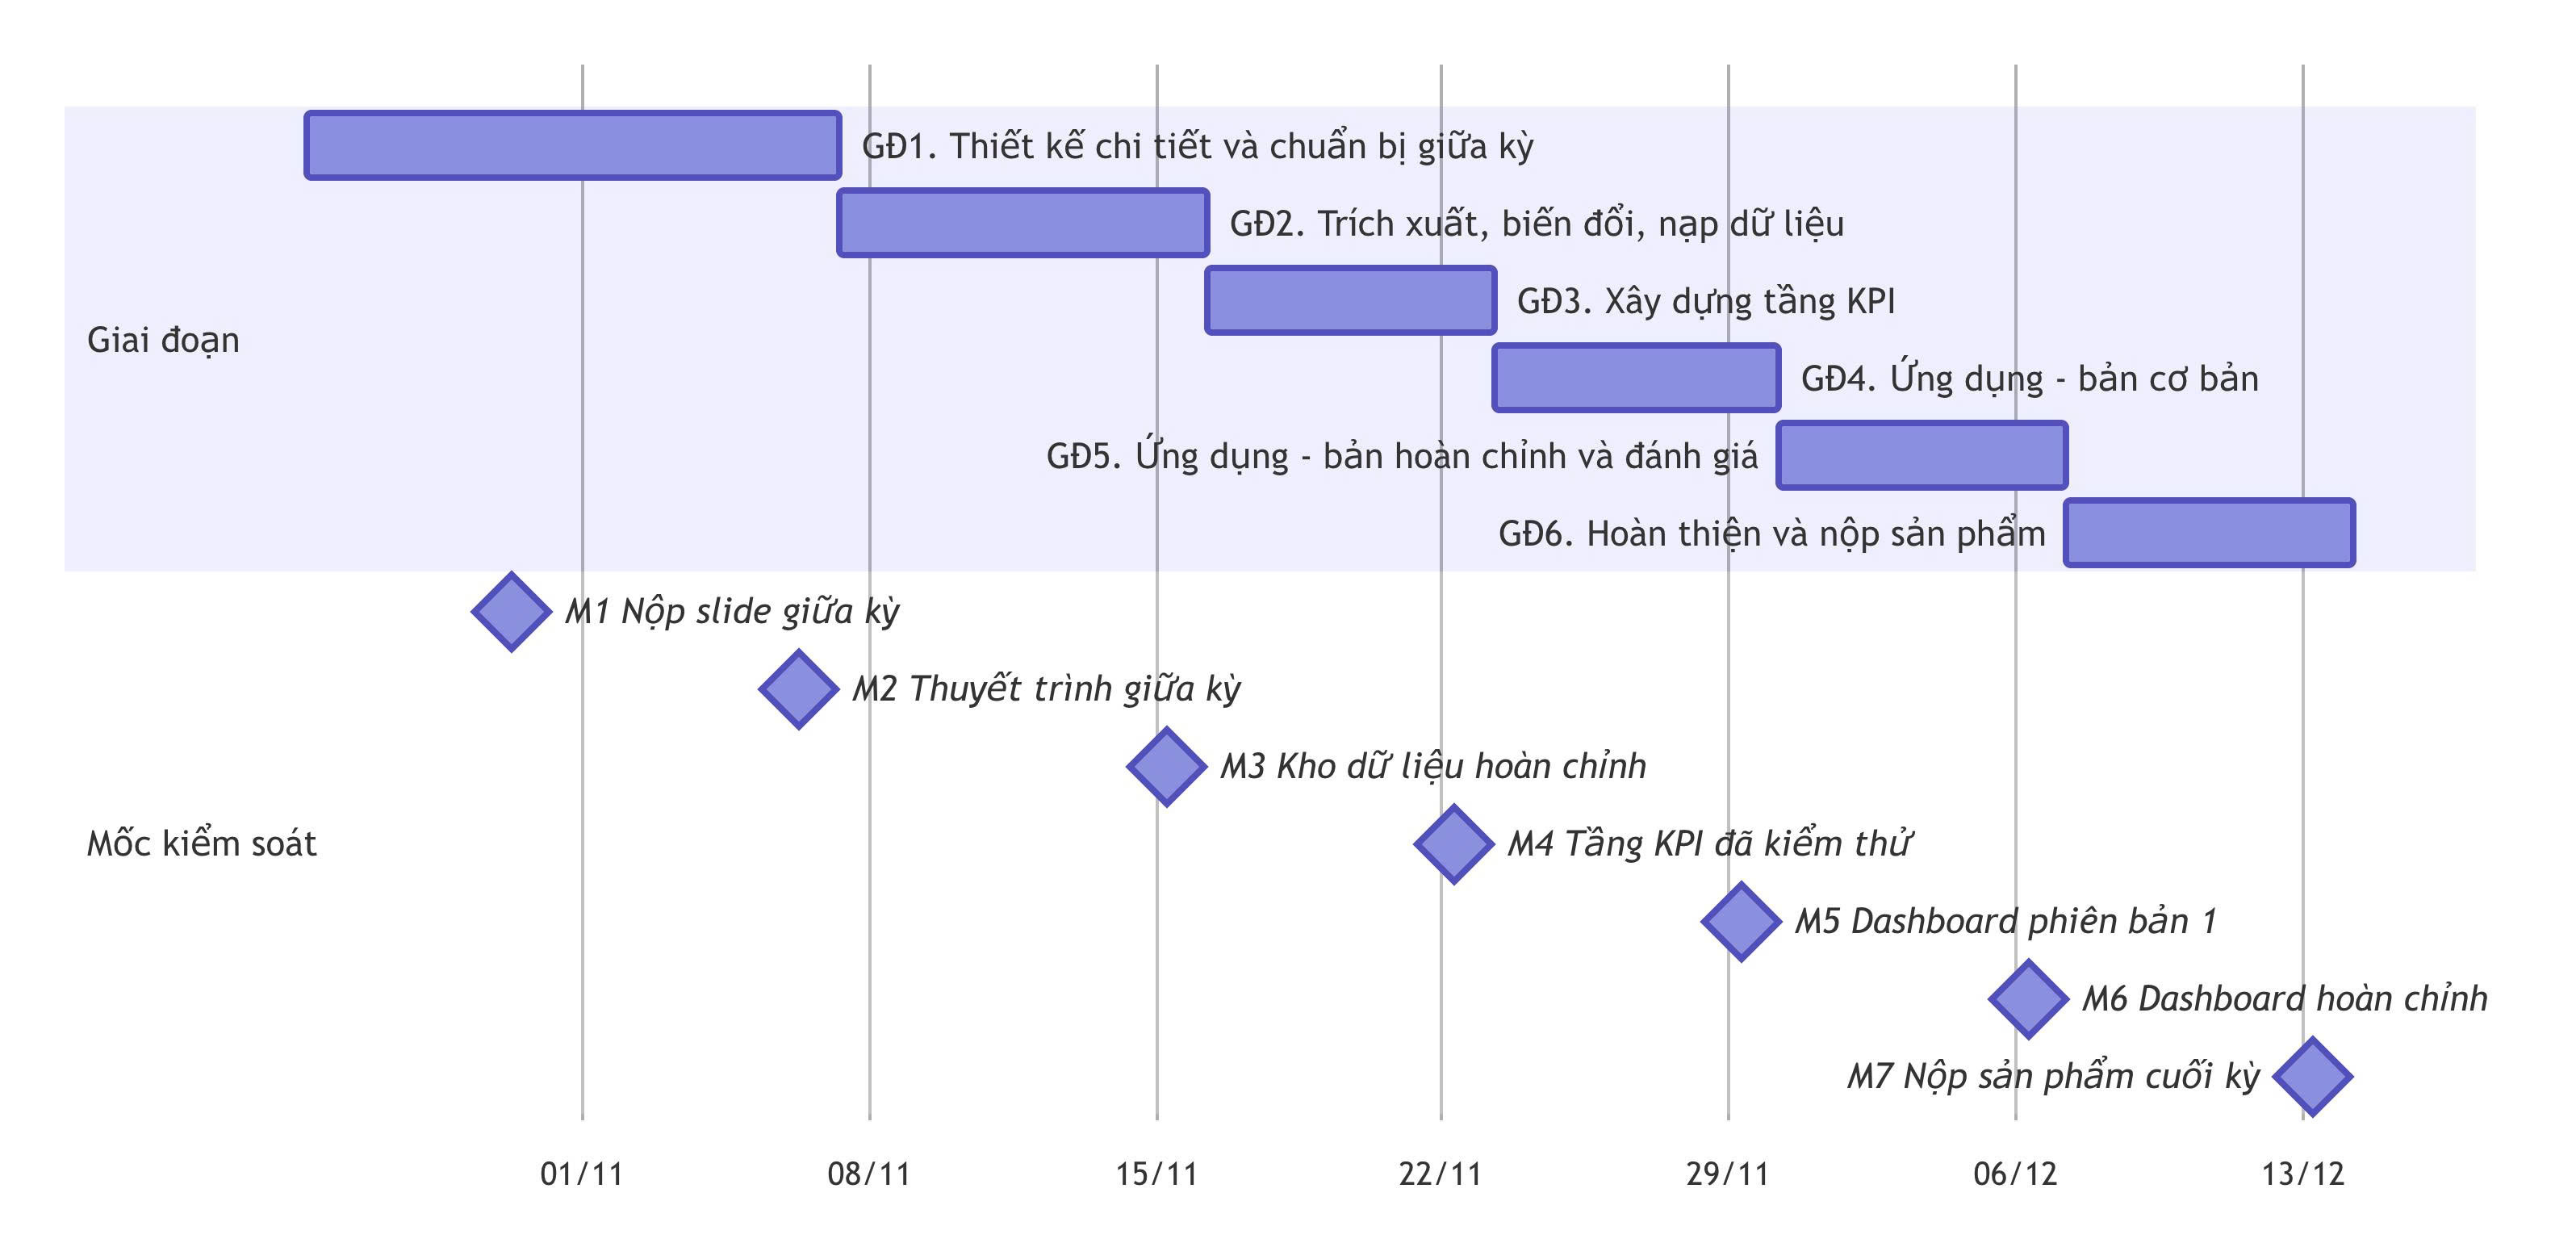
\includegraphics[width=0.9\textwidth]{image/Hien/Gantt_Chart.jpg}
    \caption{Biểu đồ Gantt kế hoạch thực hiện dự án}
    \label{fig:gantt}
\end{figure}

% ---------------------------------------------------------------------
\subsection{Phân công nhiệm vụ}
\label{subsec:phan-cong}

Nhóm phân công theo vai trò kỹ thuật, bám theo các tầng kiến trúc ở mục~3.3
(Bảng~\ref{tab:phan-cong}). Mỗi tầng có một thành viên chịu trách nhiệm chính và một
thành viên hỗ trợ, để mọi phần việc đều được rà soát chéo và có người tiếp quản khi
cần. Các sản phẩm tài liệu (báo cáo, slide, video) do cả nhóm cùng thực hiện; mỗi
thành viên trình bày phần mình phụ trách nhưng nắm được toàn bộ luồng dữ liệu, nhằm
bảo đảm đóng góp đồng đều trong các buổi thuyết trình.

% TODO: Nhóm xác nhận lại phân công vai trò bên dưới trước khi nộp.
\begin{table}[htbp]
    \centering
    \small
    \caption{Phân công vai trò và trách nhiệm}
    \label{tab:phan-cong}
    \begin{tabularx}{\textwidth}{|>{\raggedright\arraybackslash}p{2.6cm}
                                 |>{\raggedright\arraybackslash}p{2.4cm}
                                 |>{\raggedright\arraybackslash}X
                                 |>{\raggedright\arraybackslash}p{3.0cm}|}
        \hline
        \textbf{Thành viên} & \textbf{Vai trò} & \textbf{Trách nhiệm chính}
            & \textbf{Hỗ trợ} \\
        \hline
        Bùi Trọng Hiển
            & Data Engineer
            & Trích xuất dữ liệu từ BigQuery; biến đổi dữ liệu (làm phẳng, dựng phiên,
              chuẩn hóa kênh, làm sạch); nhật ký chất lượng dữ liệu; tự động hóa quy
              trình ETL
            & Nạp dữ liệu; kiểm thử mốc M3 \\
        \hline
        Nguyễn Xuân Huy Hoàng
            & Data Warehouse \& KPI Engineer
            & Thiết kế chi tiết lược đồ hình sao; nạp kho dữ liệu; cài đặt và kiểm
              thử tầng KPI; tối ưu truy vấn; chức năng truy vết số liệu
            & Bộ quy tắc gom kênh; kết nối dashboard với tầng KPI \\
        \hline
        Trần Vĩnh Dũng
            & Application Developer
            & Thiết kế giao diện và phát triển dashboard; các chức năng bộ lọc, so
              sánh, phễu, drill-down, phân khúc, cảnh báo theo ngưỡng và mô phỏng
              kịch bản
            & Kiểm thử tổng thể; biên tập video demo \\
        \hline
        Cả nhóm
            & --
            & Báo cáo, slide giữa kỳ và cuối kỳ; đánh giá hệ thống; video demo;
              thuyết trình
            & -- \\
        \hline
    \end{tabularx}
\end{table}

% ---------------------------------------------------------------------
\subsection{Công nghệ và công cụ}
\label{subsec:cong-nghe}

Công nghệ cho tầng nguồn và tầng xử lý đã được xác định. Với tầng kho dữ liệu và tầng
ứng dụng, nhóm đang cân nhắc giữa hai phương án và sẽ chốt trước ngày 30/10/2026 dựa
trên các tiêu chí ở Bảng~\ref{tab:cong-nghe}. Đánh giá sơ bộ cho thấy DuckDB phù hợp
với quy mô dữ liệu ba tháng và dễ chia sẻ giữa các thành viên, trong khi Streamlit linh
hoạt hơn cho chức năng mô phỏng kịch bản và truy vết số liệu; quyết định cuối cùng sẽ
dựa trên kết quả trích xuất thử ở giai đoạn~1.

\begin{table}[htbp]
    \centering
    \small
    \caption{Công nghệ dự kiến và tiêu chí lựa chọn}
    \label{tab:cong-nghe}
    \begin{tabularx}{\textwidth}{|>{\raggedright\arraybackslash}p{2.4cm}
                                 |>{\raggedright\arraybackslash}p{3.0cm}
                                 |>{\raggedright\arraybackslash}X
                                 |>{\raggedright\arraybackslash}p{1.8cm}|}
        \hline
        \textbf{Tầng} & \textbf{Công nghệ} & \textbf{Tiêu chí lựa chọn}
            & \textbf{Trạng thái} \\
        \hline
        Nguồn dữ liệu & Google BigQuery
            & Nơi lưu trữ sẵn tập dữ liệu GA4 & Đã chốt \\
        \hline
        Trích xuất và biến đổi & Python (pandas), SQL
            & Xử lý tốt cấu trúc lồng nhau; dễ tự động hóa và kiểm thử & Đã chốt \\
        \hline
        Kho dữ liệu & PostgreSQL hoặc DuckDB
            & Hiệu năng truy vấn phân tích; dễ triển khai và chia sẻ giữa các thành
              viên; tương thích với công cụ dashboard & Chốt trước 30/10 \\
        \hline
        Ứng dụng hỗ trợ ra quyết định & Power BI hoặc Streamlit
            & Mức độ tương tác cho người ra quyết định, đặc biệt với ngưỡng cảnh báo
              do người dùng cấu hình, mô phỏng kịch bản và truy vết số liệu; khả năng
              drill-down; thuận tiện khi demo & Chốt trước 30/10 \\
        \hline
        Cộng tác & GitHub, Overleaf, Google Drive
            & Quản lý mã nguồn và rà soát chéo; soạn báo cáo chung; lưu trữ tài liệu
            & Đã chốt \\
        \hline
    \end{tabularx}
\end{table}
\newpage
% ---------------------------------------------------------------------
\subsection{Quản lý rủi ro}
\label{subsec:rui-ro}

Bảng~\ref{tab:rui-ro} liệt kê các rủi ro chính có thể ảnh hưởng đến tiến độ và chất
lượng, cùng phương án phòng ngừa.

\begin{table}[htbp]
    \centering
    \small
    \caption{Các rủi ro chính và phương án xử lý}
    \label{tab:rui-ro}
    \begin{tabularx}{\textwidth}{|>{\raggedright\arraybackslash}p{5.2cm}
                                 |>{\raggedright\arraybackslash}p{2.1cm}
                                 |>{\raggedright\arraybackslash}X|}
        \hline
        \textbf{Rủi ro} & \textbf{Mức độ} & \textbf{Phương án xử lý} \\
        \hline
        Chất lượng dữ liệu nguồn làm sai lệch KPI
            & Cao & Kiểm chứng sớm và ghi nhật ký chất lượng dữ liệu \\
        \hline
        Trễ tiến độ giữa các giai đoạn
            & Trung bình & Theo dõi theo mốc; phát triển song song trên dữ liệu mẫu \\
        \hline
        Hiệu năng truy vấn chưa đáp ứng tính tương tác
            & Trung bình & Tối ưu truy vấn và dùng bảng tổng hợp \\
        \hline
        Phạm vi công việc vượt khả năng
            & Trung bình & Ưu tiên các chức năng cốt lõi trước \\
        \hline
        Thành viên quá tải vào cuối kỳ
            & Cao & Dành thời gian dự phòng; rà soát chéo để hỗ trợ lẫn nhau \\
        \hline
    \end{tabularx}
\end{table}

% ---------------------------------------------------------------------
\subsection{Phối hợp và theo dõi tiến độ}
\label{subsec:phoi-hop}

Để bảo đảm kế hoạch được thực hiện đúng, nhóm áp dụng các nguyên tắc sau:
\begin{itemize}
    \item \textbf{Họp định kỳ hằng tuần:} cập nhật tiến độ so với các mốc kiểm soát,
          xác định vướng mắc và điều chỉnh phân công khi có giai đoạn bị chậm.
    \item \textbf{Quản lý mã nguồn:} mỗi thành viên làm việc trên nhánh riêng trên
          GitHub; mã nguồn được thành viên hỗ trợ rà soát trước khi gộp vào nhánh
          chính.
    \item \textbf{Kiểm soát theo mốc:} mỗi mốc M1--M7 được nghiệm thu theo tiêu chí ở
          Bảng~\ref{tab:moc} trước khi chuyển giai đoạn.
    \item \textbf{Ghi nhận đóng góp:} công việc và mức độ hoàn thành của từng thành
          viên được ghi lại hằng tuần, làm cơ sở cho phụ lục báo cáo hoạt động nhóm
          (Teamwork report) trong báo cáo cuối kỳ.
\end{itemize}
\pagebreak
\section{Kết luận}
\label{sec:ketluan}

\subsection{Tổng kết kết quả thực hiện}
\label{sec:summary}

Đồ án đã xây dựng và vận hành hoàn chỉnh luồng xử lý dữ liệu GA4 từ khâu thu thập đến trực quan hóa: publisher phát lại các sự kiện theo đúng trình tự thời gian, Pub/Sub Emulator đóng vai trò hàng đợi trung gian cục bộ và Apache Beam xử lý dữ liệu thông qua DirectRunner. Sau khi chuẩn hóa, các tệp JSONL được nạp lên BigQuery Sandbox để dbt triển khai các tầng staging, mô hình sao (core star schema), data marts và các khung nhìn chỉ số (KPI views). Dashboard Streamlit khai thác trực tiếp các bảng tổng hợp này nhằm bảo đảm tính nhất quán thay vì tự tính toán một bộ chỉ số riêng lẻ.\medskip

Về mặt tổ chức dữ liệu, mô hình kho gồm 4 bảng fact dùng chung 8 bảng dimension với mức độ chi tiết (grain) được định nghĩa rõ ràng. Lớp tổng hợp chỉ lưu trữ các số đo có tính cộng được để tránh sai số khi tính toán lại các tỷ lệ ở nhiều chiều phân tích. Về mặt nghiệp vụ, mỗi phiên được xác định dựa trên cặp định danh người dùng và mã phiên, đồng thời gắn ngày theo sự kiện phát sinh đầu tiên. Giao dịch hợp lệ phải là sự kiện \texttt{purchase} có mã giao dịch thực, doanh thu dương và được khử trùng bằng cách giữ lại bản ghi sớm nhất. Khi phân bổ nguồn truy cập, hệ thống ưu tiên lấy nguồn cấp phiên và chỉ dùng nguồn cấp người dùng để thay thế nếu phiên không ghi nhận thông tin nguồn.\medskip

Kết quả kiểm thử thực tế cho thấy các thành phần trong kiến trúc đã phối hợp trơn tru: 100 sự kiện từ nguồn dữ liệu công khai được truyền qua emulator và DirectRunner, nạp đầy đủ vào tầng dữ liệu thô, dựng thành công 19 mô hình dbt, vượt qua toàn bộ 5 bài kiểm thử dữ liệu và hiển thị chính xác lên dashboard Streamlit. Toàn bộ luồng xử lý cũng đã được đóng gói và tái lập thành công trong môi trường Docker trên WSL, đi kèm cơ chế giám sát giới hạn tài nguyên và dọn dẹp tiến trình tự động. Quá trình vận hành trên BigQuery Sandbox luôn nằm trong hạn mức miễn phí nhờ áp dụng kiểm tra trước (dry-run), giới hạn dung lượng quét cho từng loại truy vấn và theo dõi mức sử dụng trên toàn dự án.\medskip

Tuy nhiên, các kết quả kiểm chứng hiện tại mới chỉ dừng ở mức nguyên mẫu (prototype) và chưa phản ánh đầy đủ hiệu năng trên toàn bộ tập dữ liệu lớn. Do lô dữ liệu thử nghiệm (mini-batch) không phát sinh giao dịch mua hàng hay thông tin mặt hàng, luồng xử lý doanh thu vẫn cần được kiểm thử thêm trên một lô dữ liệu riêng có kiểm soát. Bên cạnh đó, DirectRunner và Pub/Sub Emulator chỉ phục vụ mục đích kiểm thử cục bộ chứ chưa thay thế được hạ tầng lưu trữ và xử lý phân tán bền vững, còn tệp xuất CSV cho Looker Studio mới chỉ đáp ứng nhu cầu báo cáo tĩnh (snapshot) thay vì kết nối dữ liệu trực tiếp.\medskip

\subsection{Hướng mở rộng hệ thống}
\label{sec:extensions}

Các dịch vụ và giải pháp có liên quan đến tài khoản thanh toán (Billing Project) được tách riêng trong mục này do nằm ngoài phạm vi vận hành miễn phí hiện tại.\medskip

Khi cần mở rộng quy mô xử lý dữ liệu hoặc chuyển sang vận hành trên hạ tầng đám mây được quản lý toàn phần, hệ thống có thể nâng cấp tầng thu thập lên Cloud Pub/Sub, tầng xử lý lên Dataflow và sử dụng Cloud Storage làm vùng lưu trữ trung gian. Quá trình chuyển đổi này đòi hỏi chuẩn bị đầy đủ về hạn mức tài nguyên (quota), phân quyền IAM, cấu hình bucket, vòng đời tác vụ (job lifecycle) và quản lý chi phí, thay vì xem như các thành phần đã sẵn có trong bản nguyên mẫu. Song song đó, cần bổ sung mô hình dữ liệu cho chi phí quảng cáo và chi phí vận hành thực tế để có cơ sở tính toán chính xác các chỉ số như ROAS hay CPA.\medskip

Đối với nhu cầu báo cáo nâng cao, tài liệu kỹ thuật của Looker Studio chỉ ra rằng trình kết nối BigQuery trực tiếp yêu cầu một dự án có gắn tài khoản thanh toán cùng quyền đọc dữ liệu và thực thi truy vấn tương ứng \parencite{looker-bigquery}. Vì vậy, nếu cần cập nhật báo cáo theo thời gian thực, doanh nghiệp cần thiết lập dự án hợp lệ và kiểm soát chặt chẽ dung lượng quét của dashboard; phương án xuất tệp CSV từ Sandbox hiện tại chỉ là giải pháp tạm thời phù hợp với phạm vi miễn phí chứ chưa thể thay thế hoàn toàn kết nối tự động liên tục.\medskip

Cuối cùng, khi khối lượng dữ liệu và yêu cầu nghiệp vụ gia tăng, kiến trúc hệ thống cần tiếp tục hoàn thiện theo hướng nạp dữ liệu tăng dần (incremental load) thay cho nạp lại toàn bộ (full-refresh), thiết lập chính sách lưu trữ dài hạn, xây dựng cơ chế khôi phục khi bảng trên Sandbox hết hạn, cũng như kiểm chứng lại toàn bộ luồng doanh thu trên các lô dữ liệu có phát sinh giao dịch thực tế. Mọi bước mở rộng về hạ tầng đều cần đi kèm quy trình kiểm thử tương đương trên dữ liệu mới thay vì chỉ dựa vào kết quả của lô thử nghiệm nhỏ hiện tại.\medskip

% REFERENCES
\pagebreak
\nocite{*}
\printbibliography[
  heading=bibintoc,
  title={Tài liệu tham khảo}
]
\end{document}
